%% Chapter 5: Planar Graphs
%% Status: drafted.
%%
%% Integrated from planar-graphs-notes.tex (kept in material/notes/ for
%% reference).  All figures are drawn in TikZ except fig:planar-gadget, the
%% crossover gadget of Garey-Johnson-Stockmeyer, which has to be copied from
%% the paper or the slides rather than guessed: it is a finite case check and
%% a wrong graph would look right.

\chapter{Planar Graphs}
\label{ch:planar}

A graph is planar if it can be drawn in the plane without edges crossing.
That is a purely topological condition, and at first sight it has nothing to
do with algorithms. It turns out to be one of the most algorithmically
consequential structural restrictions we know.

\begin{goals}
  \poolgoal{give and prove Euler's formula}
  \poolgoal{show that $m \le 3n-6$ and that the average degree is below $6$}
  \poolgoal{define graph minors and state Kuratowski's theorem}
  \poolgoal{show that planar graphs are $5$-colourable}
  \poolgoal{show that $K_{3,3}$ is non-planar in an elementary way}
  \goalitem{explain how planarity can be tested in $\bigoh{n^3}$ time using segments and interlacement}
  \poolgoal{state the planar separator theorem}
  \poolgoal{show that \MIS{} can be solved in $2^{\bigoh{\sqrt n}}$ time on planar graphs}
  \poolgoal{show that $3$-colouring is NP-hard for planar graphs}
\end{goals}

%==============================================================================
\section{Introduction}
%==============================================================================

There are two separate reasons to care, and this chapter is organised around
them.

The first is that planarity is a real constraint that real inputs satisfy.
Road networks, printed circuit boards, floor plans, and many geometric meshes
are planar or nearly so. If your input is planar you would like to know it,
and you would like to exploit it. So the first algorithmic question is simply:
\emph{given a graph, can we decide efficiently whether it is planar?} The
answer is yes, and remarkably it can be done in linear time; we will study a
slower but far more instructive $\bigoh{n^3}$ algorithm, because the ideas in
it --- cycles, segments, interlacement --- are the ideas everybody uses.

The second reason is deeper. Planar graphs cannot be tangled: they have small
\emph{balanced separators}. Deleting only $\bigoh{\sqrt{n}}$ vertices splits a
planar graph into pieces none of which is larger than a constant fraction of
the whole. This is the Planar Separator Theorem, and it is the engine behind a
whole family of divide-and-conquer algorithms. We will use it to solve
\textsc{Maximum Independent Set} --- NP-hard in general, and still NP-hard on
planar graphs --- in time $2^{\bigoh{\sqrt{n}}}$ rather than $2^{\bigoh{n}}$.
That is not polynomial, but on a graph with $10\,000$ vertices it is the
difference between impossible and routine.

We close by looking at what \emph{stays} hard. Most NP-hard graph problems
remain NP-hard when restricted to planar inputs, and we prove this for
$3$-colouring. There are a few notable exceptions, and \textsc{Clique} is one
of them --- for a reason that is a one-line consequence of the structure theory
in Section~\ref{sec:planar-basics}.

\begin{itemize}[nosep]
  \item Section~\ref{sec:planar-basics}: Euler's formula and its consequences, minors,
        Kuratowski--Wagner, colouring, Fáry's theorem.
  \item Section~\ref{sec:planar-testing}: an $\bigoh{n^3}$ planarity test.
  \item Section~\ref{sec:planar-pst}: the Planar Separator Theorem.
  \item Section~\ref{sec:planar-mis}: independent set in $2^{\bigoh{\sqrt n}}$ time.
  \item Section~\ref{sec:planar-hardness}: what remains NP-hard, and what does not.
\end{itemize}

Throughout, $G = (V,E)$ is a graph with $n = |V|$ vertices and $m = |E|$ edges.

%==============================================================================
\section{Basics}\label{sec:planar-basics}
%==============================================================================

\subsection{Planar graphs, plane graphs, faces}

We must distinguish two notions that are easy to conflate, and the distinction
matters constantly in what follows.

\begin{definition}[Planar and plane]
A graph is \emph{planar} if it \emph{can} be drawn in $\R^2$ with no two edges
crossing. A \emph{plane graph} is a planar graph \emph{together with} one such
drawing: the embedding is fixed.
\end{definition}

Planarity is a property of an abstract graph; being plane is a property of a
drawing. The same planar graph has many essentially different embeddings, and
several of the quantities we are about to define --- faces, in particular ---
depend on the embedding rather than on the graph.

This cuts both ways, and the asymmetry is worth pausing on. A crossing-free
drawing \emph{proves} that a graph is planar; you can point at it. A drawing
with crossings proves nothing at all --- it may just be a bad drawing of a
perfectly planar graph. \Cref{fig:planar-vs-plane} shows the same phenomenon on
$K_{3,3}$ minus an edge: drawn one way it looks hopelessly tangled, drawn
another way it is visibly plane --- and the two drawings really are the same
graph, vertex labels and all. Establishing that a graph is \emph{not} planar
therefore needs an argument about all possible drawings at once, which is what
\cref{sec:planar-minors,sec:planar-k33warmup} are for.

\begin{definition}[Faces]
Let $G$ be a plane graph. Removing the drawing from the plane leaves a
collection of connected open regions, called the \emph{faces} of the
embedding. Exactly one of them is unbounded; it is the \emph{outer face}, and
the others are the \emph{interior faces}.
\end{definition}

\begin{figure}[ht]
\centering

\includegraphics[width=0.62\textwidth]{planar-vs-plane}
\caption{One graph --- $K_{3,3}$ minus the edge $\{3,4\}$ --- drawn twice. The
left drawing has crossings; the right one does not. Only the right drawing
carries information about the graph: a drawing with crossings never witnesses
non-planarity, it only witnesses its own clumsiness. In the right drawing the
faces are shaded, $f_1, f_2, f_3$ being the interior faces and $f_4$ the outer
one. Nothing in the left drawing corresponds to them --- faces exist only once
an embedding is fixed.}
\label{fig:planar-vs-plane}
\end{figure}

A useful bookkeeping fact, with one exception that will bite us if we ignore
it: \emph{every edge is incident to exactly two faces} --- except a
\emph{bridge} (an edge whose removal disconnects its component), which has the
same face on both sides. The right way to think about it, and the way that
makes the counting arguments below uniform, is to count \emph{edge-sides}:
every edge has two sides, and each side lies on exactly one face. For a
non-bridge these are two different faces; for a bridge they are the same face
twice.

\begin{figure}[ht]
\centering

\includegraphics[width=0.5\textwidth]{planar-bridge}
\caption{The highlighted edge is a bridge: deleting it disconnects the graph.
Every other edge here has two different faces on its two sides. The bridge does
not: walk around it and you stay in the outer face the whole way, so it borders
one face rather than two.}
\label{fig:planar-bridge}
\end{figure}

\subsection{Euler's formula}\label{sec:planar-euler}

Every quantitative statement about planar graphs in this chapter descends from
one identity, which Euler found for polyhedra in 1750. It relates the three
things a plane drawing has.

\begin{theorem}[Euler]\label{thm:planar-euler}
Let $G$ be a connected plane graph with $n \ge 1$ vertices, $m$ edges and $f$
faces. Then
\[
  n + f = m + 2 .
\]
\end{theorem}

\begin{proof}
By induction on $m$.

\emph{Base case $m = 0$.} A connected graph with no edges is a single vertex,
so $n = 1$, and the drawing leaves the whole plane as one face, $f = 1$. Indeed
$1 + 1 = 0 + 2$.

\emph{Inductive step.} Let $m \ge 1$ and assume the formula for all connected
plane graphs with fewer edges. We distinguish two cases, and we must check
that they are exhaustive.

\begin{itemize}
  \item \textbf{$G$ contains a cycle.} Let $e$ be an edge on that cycle. Then
        $e$ is not a bridge, so the two sides of $e$ belong to two
        \emph{different} faces. Deleting $e$ keeps the graph connected and
        merges those two faces into one. So the new graph has $n' = n$,
        $m' = m - 1$ and $f' = f - 1$, and it is still a connected plane graph.
        By induction $n' + f' = m' + 2$, that is $n + f - 1 = m - 1 + 2$, which
        rearranges to $n + f = m + 2$.
  \item \textbf{$G$ has a vertex $v$ of degree $1$.} Delete $v$ and its edge.
        The graph stays connected, no faces merge or split (the pendant edge
        had the same face on both sides), so $n' = n - 1$, $m' = m - 1$,
        $f' = f$. By induction $n - 1 + f = m - 1 + 2$, i.e.\ $n + f = m + 2$.
\end{itemize}

These two cases cover everything: if $G$ has no vertex of degree $1$ and at
least one edge, then --- being connected --- it has minimum degree at least
$2$, and a graph with minimum degree at least $2$ contains a cycle. (Walk
forward without immediately reusing the edge you came on; since the graph is
finite you must eventually revisit a vertex, and the walk between the two
visits is a cycle.)
\end{proof}

\begin{figure}[ht]
\centering

\includegraphics[width=0.72\textwidth]{planar-euler-induction}
\caption{The two inductive steps. Left: $e$ lies on a cycle, so its two sides
belong to different faces and deleting it merges them --- $m$ and $f$ both drop
by one. Right: $e$ hangs off a degree-$1$ vertex, so both its sides lie on the
same face and deleting the vertex changes no face --- $n$ and $m$ both drop by
one.}
\label{fig:planar-euler-induction}
\end{figure}

\begin{intuition}
Euler's formula says that a plane drawing has no slack: the three quantities
$n$, $m$, $f$ are locked together. This is what turns a topological hypothesis
(``drawable without crossings'') into a combinatorial one (``not too many
edges''), and every quantitative statement in this section is an application of
that translation.

Notice also that $n$ and $m$ do not depend on the drawing, so neither does $f$:
\emph{every} plane embedding of a given connected planar graph has the same
number of faces. That is already a non-trivial corollary.
\end{intuition}

\subsection{Consequences: edge counts and low-degree vertices}\label{sec:planar-sparsity}

Euler's formula alone does not bound $m$; we also need that faces cannot be
too small. That is where simplicity comes in.

\begin{corollary}\label{cor:planar-3n-6}
Let $G$ be a connected plane graph with no parallel edges and no self-loops
and with $n > 2$. Then
\[
  m \;\le\; 3n - 6 .
\]
\end{corollary}

\begin{proof}
Count edge-sides in two ways. Every face is bounded by at least three
edge-sides: with no loops and no parallel edges and at least three vertices,
no face can be enclosed by one or two edge-sides. Summing over faces gives a
total of at least $3f$ edge-sides. On the other hand every edge has exactly two
sides, so the total is exactly $2m$. Hence
\[
  3f \le 2m, \qquad\text{i.e.}\qquad f \le \tfrac{2}{3}m .
\]
Substituting into Euler's formula $f = m + 2 - n$ gives
\[
  m + 2 - n \;\le\; \tfrac{2}{3} m
  \qquad\Longrightarrow\qquad
  \tfrac{1}{3} m \;\le\; n - 2
  \qquad\Longrightarrow\qquad
  m \le 3n - 6 . \qedhere
\]
\end{proof}

\begin{corollary}[$K_5$ is not planar]\label{cor:planar-k5}
The complete graph $K_5$ is not planar.
\end{corollary}

\begin{proof}
$K_5$ has $n = 5$ and $m = 10$, but $3n - 6 = 9 < 10$.
\end{proof}

This is the first genuinely useful thing we can do: a purely arithmetic
certificate of non-planarity. It does \emph{not} work for $K_{3,3}$, which has
$n = 6$, $m = 9 \le 12$; there one has to use that bipartite plane graphs have
faces of length at least four, giving $m \le 2n - 4 = 8 < 9$. Try it as an
exercise. A completely different and much more instructive proof, which is
really the planarity-testing algorithm run by hand, is given in
Section~\ref{sec:planar-k33warmup}.

\begin{corollary}[Sparse graphs have sparse spots]\label{cor:planar-deg5}
Every plane graph with no parallel edges and no self-loops has a vertex of
degree at most $5$.
\end{corollary}

\begin{proof}
For $n \le 2$ this is trivial, so assume $n > 2$ and, by taking a component,
that $G$ is connected. The average degree is
\[
  \frac{1}{n}\sum_{v \in V} \dg(v) = \frac{2m}{n}
  \;\le\; \frac{2(3n-6)}{n} = 6 - \frac{12}{n} \;<\; 6 .
\]
A finite set of integers with average less than $6$ must contain an element
that is at most $5$.
\end{proof}

\begin{intuition}
Corollary~\ref{cor:planar-deg5} is small but it is the workhorse of the whole
subject. It says planar graphs always have a cheap place to start an
induction. Every colouring result below is ``delete a low-degree vertex,
colour the rest, put the vertex back'', and the only reason that strategy is
available at all is this corollary. Note too that it is inherited: every
subgraph of a planar graph is planar, so the induction never leaves the class.
\end{intuition}

\subsection{Minors and the Kuratowski--Wagner theorem}\label{sec:planar-minors}

Corollary~\ref{cor:planar-k5} suggests a plan: characterise planarity by forbidden
sub-structures. The right notion of sub-structure is not the subgraph but the
minor.

\begin{definition}[Minor]
A graph $H$ is a \emph{minor} of a graph $G$ if $H$ can be obtained from $G$ by
a sequence of the following operations:
\begin{itemize}[nosep]
  \item \emph{edge deletion},
  \item \emph{vertex deletion} (together with its incident edges),
  \item \emph{edge contraction}: replace an edge $\{u,v\}$ by a single new
        vertex adjacent to all former neighbours of $u$ and of $v$.
\end{itemize}
\end{definition}

\begin{figure}[ht]
\centering

\includegraphics[width=0.9\textwidth]{planar-contraction}
\caption{Contracting the edge $\{d,e\}$. The new vertex $de$ inherits every
neighbour of $d$ and every neighbour of $e$; nothing else about the graph
changes. Note what contraction is not: it is not deletion of a vertex, and the
rest of the graph --- here drawn as the two blobs --- is untouched.}
\label{fig:planar-contraction}
\end{figure}

The single most important property, and the reason minors are the right notion
here, is this:

\begin{observation}\label{obs:planar-minor-closed}
Every minor of a planar graph is planar.
\end{observation}

\begin{proof}[Proof idea]
Each of the three operations can be performed directly on a drawing. Deleting
an edge or a vertex only erases ink. Contracting an edge $\{u,v\}$ can be done
by sliding $u$ along the drawn edge towards $v$, dragging its other edges with
it; since we slide along a curve that is already crossing-free, no crossings
are created.
\end{proof}

So the class of planar graphs is \emph{minor-closed}, and any minor of a planar
graph is a legitimate certificate: exhibiting a non-planar minor proves
non-planarity. Two small examples of what minors can express:

\begin{example}
$K_3$ (a triangle) is a minor of $G$ if and only if $G$ contains a cycle.
Indeed, contracting a cycle of length $\ell > 3$ once shortens it to length
$\ell - 1$, so any cycle can be contracted down to a triangle; conversely a
triangle minor certainly requires a cycle to have been present.
\end{example}

\begin{theorem}[Kuratowski, Wagner]\label{thm:planar-kuratowski}
A graph is planar if and only if it has neither $K_5$ nor $K_{3,3}$ as a minor.
\end{theorem}

We do not prove this. One direction is easy and worth stating explicitly: if
$G$ is planar then by Observation~\ref{obs:planar-minor-closed} all its minors are
planar, and $K_5$ (Corollary~\ref{cor:planar-k5}) and $K_{3,3}$ (the exercise above)
are not. The hard direction is that these two obstructions are the \emph{only}
ones, which is a genuinely deep statement --- it is the prototype for
Robertson and Seymour's graph minor theorem, which says every minor-closed
class has a finite set of forbidden minors.

\begin{figure}[ht]
\centering
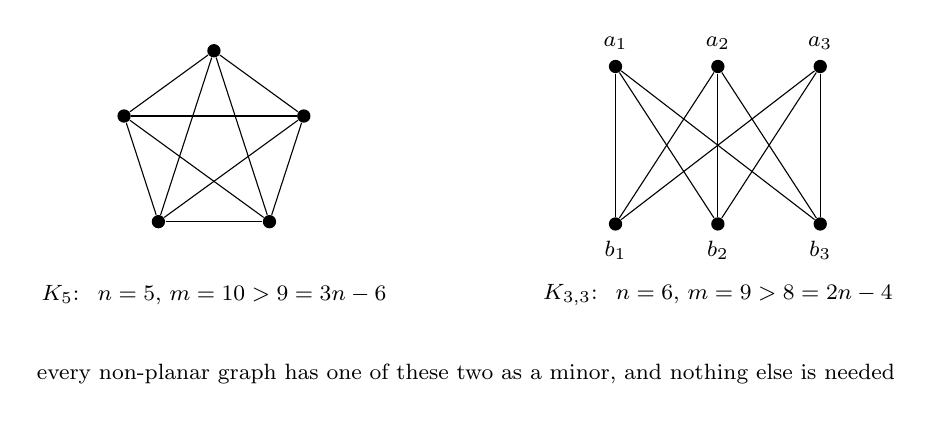
\begin{tikzpicture}[scale=1.0,
    vtx/.style={circle,fill=black,inner sep=1.7pt},
    every node/.style={font=\footnotesize}]
  % K5
  \foreach \i in {1,...,5}{ \node[vtx] (k\i) at ({90+72*\i}:1.2) {}; }
  \foreach \i in {1,...,5}{ \foreach \j in {1,...,5}{
    \ifnum\i<\j \draw (k\i)--(k\j); \fi }}
  \node at (0,-1.9) {$K_5$: \ $n=5$, $m=10 > 9 = 3n-6$};
  % K33
  \begin{scope}[xshift=6.4cm]
    \foreach \i in {1,2,3}{
      \node[vtx,label=above:$a_\i$] (a\i) at (1.3*\i-2.6,1.0) {};
      \node[vtx,label=below:$b_\i$] (b\i) at (1.3*\i-2.6,-1.0) {};
    }
    \foreach \i in {1,2,3}{ \foreach \j in {1,2,3}{ \draw (a\i)--(b\j); }}
    \node at (0,-1.9) {$K_{3,3}$: \ $n=6$, $m=9 > 8 = 2n-4$};
  \end{scope}
  \node[align=center] at (3.2,-2.9)
    {every non-planar graph has one of these two as a minor, and nothing else
     is needed};
\end{tikzpicture}
\caption{The two forbidden minors.}
\label{fig:planar-k5k33}
\end{figure}

\begin{figure}[ht]
\centering
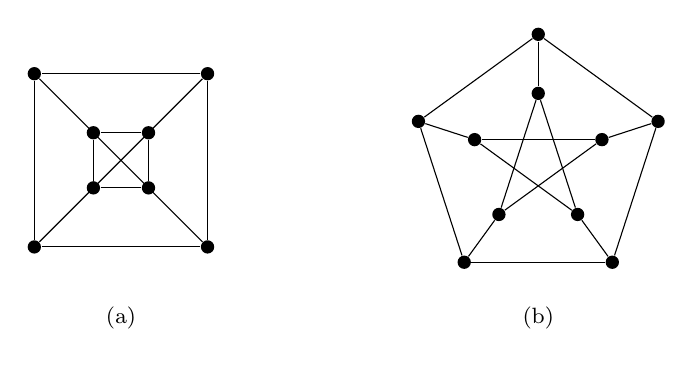
\begin{tikzpicture}[scale=1.0,
    vtx/.style={circle,fill=black,inner sep=1.7pt},
    every node/.style={font=\footnotesize}]
  % (a) the 3-cube, drawn with crossings
  \foreach \i/\x/\y in {1/0/0, 2/2.2/0, 3/2.2/2.2, 4/0/2.2}{
    \node[vtx] (o\i) at (\x,\y) {};
  }
  \foreach \i/\x/\y in {1/0.75/0.75, 2/1.45/0.75, 3/1.45/1.45, 4/0.75/1.45}{
    \node[vtx] (n\i) at (\x,\y) {};
  }
  \draw (o1)--(o2)--(o3)--(o4)--(o1);
  \draw (n1)--(n2)--(n3)--(n4)--(n1);
  \draw (o1)--(n3) (o2)--(n4) (o3)--(n1) (o4)--(n2);
  \node at (1.1,-0.9) {(a)};
  % (b) the Petersen graph
  \begin{scope}[xshift=6.4cm,yshift=1.1cm]
    \foreach \i in {1,...,5}{
      \node[vtx] (p\i) at ({90+72*\i}:1.6) {};
      \node[vtx] (q\i) at ({90+72*\i}:0.85) {};
      \draw (p\i)--(q\i);
    }
    \foreach \i [evaluate=\i as \j using {int(mod(\i,5)+1)}] in {1,...,5}{
      \draw (p\i)--(p\j);
    }
    \foreach \i [evaluate=\i as \j using {int(mod(\i+1,5)+1)}] in {1,...,5}{
      \draw (q\i)--(q\j);
    }
    \node at (0,-2.0) {(b)};
  \end{scope}
\end{tikzpicture}
\caption{Planar or not? Decide for each, and justify with a drawing or a
forbidden minor.}
\label{fig:planar-quiz}
\end{figure}

\begin{remark}[Why this does not give an algorithm]\label{rem:planar-no-algo}
Theorem~\ref{thm:planar-kuratowski} is a characterisation, not a procedure. To use it
directly we would have to search for a $K_5$ or $K_{3,3}$ minor, and the number
of candidate minors is exponential --- we would have to choose which vertices
get merged into which branch set. This is exactly why
Section~\ref{sec:planar-testing} builds a completely different algorithm. (It is
\emph{true} that testing for a fixed minor $H$ can be done in polynomial time
by deep results of Robertson and Seymour, but that machinery is far heavier
than the problem deserves, and it came thirty years later.)
\end{remark}

\subsection{Colouring planar graphs}\label{sec:planar-colouring}

Planarity limits how tangled a graph can be, and colouring is the classical
way of measuring that. We prove what an elementary argument gives, and then say
what is true but much harder.

\begin{definition}
A \emph{$k$-colouring} of $G$ is a map $c : V \to \{1,\dots,k\}$ such that
$c(u) \neq c(v)$ for every edge $\{u,v\} \in E$. $G$ is \emph{$k$-colourable}
if such a map exists.
\end{definition}

\begin{proposition}\label{prop:planar-6col}
Every planar graph is $6$-colourable.
\end{proposition}

\begin{proof}
Induction on $|V|$. Graphs with at most $6$ vertices are trivially
$6$-colourable. Otherwise, by Corollary~\ref{cor:planar-deg5} there is a vertex $v$
with $\dg(v) \le 5$. The graph $G - v$ is planar and smaller, so by induction
it has a $6$-colouring. Now put $v$ back: its at most $5$ neighbours use at
most $5$ of the $6$ colours, so at least one colour is free for $v$.
\end{proof}

The same idea gives one colour better, but the last step needs an extra idea:
with $\dg(v) = 5$ all six colours may be blocked, so we must arrange for two of
$v$'s neighbours to share a colour \emph{before} we remove $v$.

\begin{theorem}\label{thm:planar-5col}
Every planar graph is $5$-colourable.
\end{theorem}

\begin{proof}
Induction on $|V|$; graphs with at most $5$ vertices are trivial. Let $G$ be
planar with $n > 5$ and let $v$ be a vertex with $\dg(v) \le 5$
(Corollary~\ref{cor:planar-deg5}).

\emph{Case 1: $\dg(v) \le 4$.} Exactly as in
Proposition~\ref{prop:planar-6col}: $5$-colour $G - v$ by induction, and give $v$ one
of the at most $4$ colours not used by its neighbours.

\emph{Case 2: $\dg(v) = 5$.} We first claim that $v$ has two non-adjacent
neighbours. Suppose not: then all five neighbours of $v$ are pairwise
adjacent, so they form a $K_5$ subgraph of $G$, contradicting
Corollary~\ref{cor:planar-k5}. Fix two non-adjacent neighbours $x$ and $y$.

Let $G'$ be obtained from $G$ by deleting $v$ and \emph{identifying} $x$ with
$y$. Then $G'$ is a minor of $G$: contract the two edges $\{v,x\}$ and
$\{v,y\}$ --- which merges $x$, $v$ and $y$ into a single vertex --- and delete
the edges from $v$ to its three other neighbours. By
Observation~\ref{obs:planar-minor-closed}, $G'$ is planar. It also has $n - 2 < n$
vertices, so by induction it has a $5$-colouring $c'$.

Pull $c'$ back to $G - v$: every vertex other than $x,y$ keeps its colour, and
both $x$ and $y$ receive the colour of the merged vertex. This is a proper
colouring of $G - v$, because the only new adjacency the identification could
have created is between $x$ and $y$ themselves, and $x,y$ are non-adjacent in
$G$ by choice.

Finally colour $v$. Its five neighbours include $x$ and $y$, which now have the
same colour, so they use at most $4$ distinct colours between them. One of the
five colours is free, and we give it to $v$.
\end{proof}

\begin{figure}[ht]
\centering

\includegraphics[width=\textwidth]{planar-5col}
\caption{Identifying two non-adjacent neighbours frees a colour for $v$. Left:
the vertex $v$ of degree $5$ with its neighbours $a$, $b$, $c$, $x$, $y$; the
shaded regions are the colour classes, and $x$ and $y$ are not adjacent. Middle:
the graph $G'$, in which $v$ has been deleted and $x$ and $y$ have been
identified into a single vertex $x = y$. Contracting along the two edges $vx$
and $vy$ keeps the drawing crossing-free, so $G'$ is still planar, and it has
two vertices fewer, so induction gives it a $5$-colouring --- visible here as
the merged colour class. Right: that colouring pulled back to $G$. Since $x$ and
$y$ came from one vertex they receive the same colour, so the five neighbours of
$v$ show at most four distinct colours between them and the fifth is free
for $v$.}
\label{fig:planar-5col}
\end{figure}

\begin{intuition}
The whole difficulty of $5$-colouring is concentrated in one place: a
degree-$5$ vertex can see five different colours, and then induction stalls.
The fix is to force a collision in advance. We are allowed to force it because
planarity guarantees that two of the neighbours are non-adjacent, so gluing
them together is harmless; and we are allowed to glue at all because gluing is
a minor operation and minors of planar graphs stay planar. Both licences come
from Section~\ref{sec:planar-basics}, which is why that section came first.
\end{intuition}

\begin{theorem}[Four Colour Theorem; Appel--Haken 1976]
Every planar graph is $4$-colourable.
\end{theorem}

We will not prove this, and neither will anybody else on a blackboard. The
proof reduces the statement to a finite but enormous case analysis --- an
unavoidable set of configurations, each checked by computer. It was the first
major theorem whose proof could not be verified by a human unaided, and it
caused a lasting argument about what a proof is for. (A formally verified
proof, machine-checked end to end, was completed by Gonthier in 2005, which
settles the correctness question if not the philosophical one.)

Note that $4$ is optimal: $K_4$ is planar and needs four colours. And in the
other direction, deciding $3$-colourability of a planar graph is NP-hard ---
we prove that in Section~\ref{sec:planar-3col}. So the complexity landscape for
planar colouring is completely mapped: $k \le 2$ easy, $k = 3$ NP-hard,
$k \ge 4$ always yes.

\subsection{Drawing with straight lines}\label{sec:planar-fary}

Our drawings so far have used curved edges freely, so it is natural to ask
whether the curves were doing any work.

\begin{theorem}[Fáry, 1936]
Every planar graph can be drawn in the plane with no crossings and with every
edge drawn as a straight line segment.
\end{theorem}

This is reassuring rather than surprising: it says the curved edges we allow
ourselves are a convenience, not a necessity. It is also the entry point to a
large research area, \emph{graph drawing}, which asks for drawings of (almost)
planar graphs that are good in various additional senses --- small area on an
integer grid, few distinct edge slopes, all faces convex, vertices at
prescribed positions, few crossings when the graph is not quite planar.

\begin{figure}[ht]
\centering

\includegraphics[width=0.6\textwidth]{planar-fary}
\caption{Fáry's theorem: curves are never necessary. Both drawings are of the
same graph --- a $4$-cycle with a hub joined to all of it --- and both are
crossing-free. The right-hand one uses curved edges; the left-hand one shows
that nothing was gained by them, since the same embedding is realisable with
straight segments. What the theorem does \emph{not} say is that the segment
endpoints can be placed anywhere convenient; how small a grid suffices is a
separate question, answered by de Fraysseix, Pach and Pollack.}
\label{fig:planar-fary}
\end{figure}

%==============================================================================
\section{Planarity testing}\label{sec:planar-testing}
%==============================================================================

\begin{quote}
\textbf{Problem.} Given a graph $G$, decide whether it is planar (and if so,
produce an embedding).
\end{quote}

Linear-time algorithms are known --- the classical ones are Hopcroft--Tarjan
(1974) and Booth--Lueker (1976), and there are several later ones that are
easier to implement. They are also fiddly, and their correctness proofs are
long. We will instead study an $\bigoh{n^3}$ algorithm going back to
Auslander--Parter and Goldstein, because it is built from ideas you can hold in
your head, and because those ideas (cycle, segments, interlacement) reappear
in the fast algorithms anyway.

As noted in Remark~\ref{rem:planar-no-algo}, Kuratowski's theorem is of no direct
help. We need a constructive strategy.

Before we start, we record the one fact about the plane that the whole
algorithm rests on.

\begin{theorem}[Jordan curve theorem]\label{thm:planar-jordan}
Let $\gamma$ be a simple closed curve in the plane. Then $\R^2 \setminus \gamma$
has exactly two connected components, one bounded and one unbounded, and
$\gamma$ is the boundary of both. In particular, any curve joining a point of
the bounded component to a point of the unbounded one meets $\gamma$.
\end{theorem}

We will use this constantly and without further comment: a cycle drawn without
crossings has an inside and an outside, and nothing gets from one to the other
without crossing it. That statement is so obviously true that it is worth
saying explicitly why we are not proving it. It is a theorem of topology, not
of combinatorics, and the honest proofs go through machinery we do not develop
here --- typically a homology or winding-number argument, or for the
polygonal special case a careful parity argument on a generic ray. None of
these techniques has anything to do with the rest of this book, and the
statement is not the kind of thing one should prove by drawing a convincing
picture: the general version covers curves far wilder than anything we will
draw. We take it on trust and get on with the algorithm.

\subsection{Warm-up: showing \texorpdfstring{$K_{3,3}$}{K33} is not planar by
hand}\label{sec:planar-k33warmup}

Before any formalism, let us do the entire thing on the smallest interesting
example. Everything the general algorithm does will appear here in miniature,
and it is worth returning to this subsection whenever the machinery in
Sections~\ref{sec:planar-segments}--\ref{sec:planar-sepcyclesec} feels abstract.

We already know from the edge count $m \le 2n-4$ that $K_{3,3}$ is not planar.
That proof is shorter than the one below, but it is a dead end: it tells us
nothing about how to \emph{search} for a drawing. The argument here is longer
and much more useful, because it is a procedure.

Write the two sides of $K_{3,3}$ as $\{a_1,a_2,a_3\}$ and $\{b_1,b_2,b_3\}$.

\paragraph{Step 1: draw a cycle.}
Start with any cycle and commit to drawing it. Take the $6$-cycle
\[
  C \;=\; a_1 \, b_1 \, a_2 \, b_2 \, a_3 \, b_3 \, a_1 ,
\]
which uses six of the nine edges of $K_{3,3}$ (check each consecutive pair: it
always joins an $a$ to a $b$, so it is indeed a cycle in the graph). Drawn
without crossings, $C$ is a closed curve, and it cuts the plane into an inside
and an outside.

\paragraph{Step 2: see what is left over.}
Three edges remain:
\[
  a_1b_2, \qquad a_2b_3, \qquad a_3b_1 .
\]
Each of them joins two vertices that are already on $C$ and touches $C$ nowhere
else. So each must be drawn either entirely inside $C$ or entirely outside
$C$ --- there is no third option, and no edge can be split between the two
regions. We have turned a drawing problem into three yes/no decisions.

\paragraph{Step 3: see which decisions clash.}
Number the positions around $C$ as
\[
  \underbrace{a_1}_{1}\;\underbrace{b_1}_{2}\;\underbrace{a_2}_{3}\;
  \underbrace{b_2}_{4}\;\underbrace{a_3}_{5}\;\underbrace{b_3}_{6},
\]
so the three leftover edges join positions
\[
  a_1b_2 : 1\text{--}4, \qquad a_2b_3 : 3\text{--}6, \qquad a_3b_1 : 5\text{--}2 .
\]
Any two of these three \emph{interleave}: going around the cycle, their
endpoints alternate. For $1\text{--}4$ and $3\text{--}6$, the order encountered
is $1,3,4,6$ --- one endpoint of the second chord lies between the endpoints of
the first, and the other lies outside. The same is true for $1\text{--}4$
against $5\text{--}2$, and for $3\text{--}6$ against $5\text{--}2$.

Two interleaving chords cannot be drawn on the same side of $C$: inside the
disc bounded by $C$, two curves whose endpoints alternate around the boundary
are forced to cross. For the moment we take this as visually evident --- it is
exactly Definition~\ref{def:planar-interlace} and Observation~\ref{obs:planar-2col} below,
where it is stated properly.

\begin{figure}[ht]
\centering
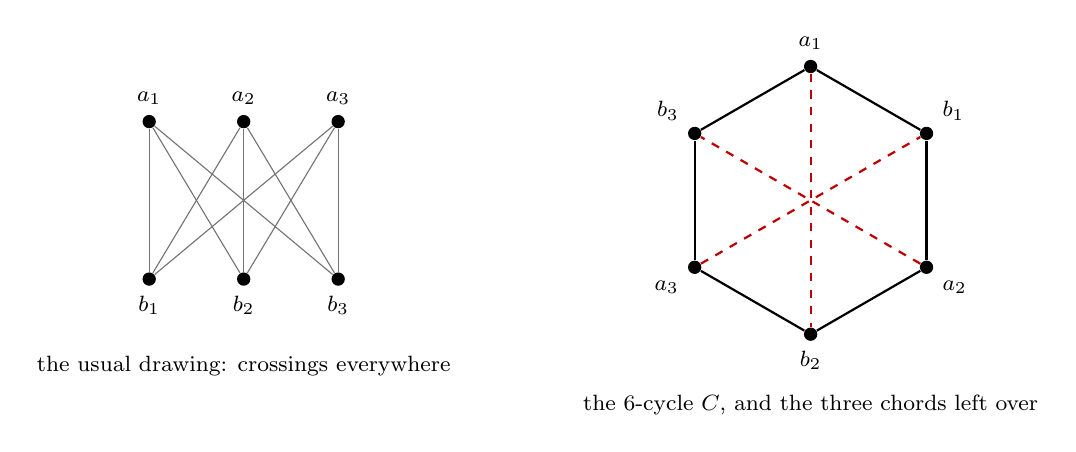
\begin{tikzpicture}[scale=1.0,
    vtx/.style={circle,fill=black,inner sep=1.7pt},
    ch/.style={red!75!black,thick,dashed},
    every node/.style={font=\footnotesize}]
  % the usual drawing
  \foreach \i in {1,2,3}{
    \node[vtx,label=above:$a_\i$] (a\i) at (1.2*\i-2.4,1.0) {};
    \node[vtx,label=below:$b_\i$] (b\i) at (1.2*\i-2.4,-1.0) {};
  }
  \foreach \i in {1,2,3}{ \foreach \j in {1,2,3}{ \draw[black!55] (a\i)--(b\j); }}
  \node at (0,-2.1) {the usual drawing: crossings everywhere};
  % the hexagon drawing
  \begin{scope}[xshift=7.2cm]
    \foreach \i/\n in {1/{a_1}, 2/{b_1}, 3/{a_2}, 4/{b_2}, 5/{a_3}, 6/{b_3}}{
      \node[vtx,label={{90-60*\i+60}:$\n$}] (h\i) at ({90-60*\i+60}:1.7) {};
    }
    \foreach \i [evaluate=\i as \j using {int(mod(\i,6)+1)}] in {1,...,6}{
      \draw[thick] (h\i)--(h\j);
    }
    \draw[ch] (h1)--(h4);
    \draw[ch] (h3)--(h6);
    \draw[ch] (h5)--(h2);
    \node at (0,-2.6) {the $6$-cycle $C$, and the three chords left over};
  \end{scope}
\end{tikzpicture}
\caption{$K_{3,3}$ redrawn around a $6$-cycle. The three remaining edges are
chords, and each must go inside or outside.}
\label{fig:planar-k33-cycle}
\end{figure}

\paragraph{Step 4: get stuck.}
Now try to make the three decisions.

\begin{itemize}
  \item Put $a_1b_2$ \emph{inside}. (Why we may assume this is the subtle
        point; see below.)
  \item $a_2b_3$ interleaves with $a_1b_2$, so it cannot also be inside. It
        must go \emph{outside}.
  \item $a_3b_1$ interleaves with $a_1b_2$, so it cannot go inside. It also
        interleaves with $a_2b_3$, so it cannot go outside. There is nowhere
        left to put it.
\end{itemize}

We are stuck, and therefore no crossing-free drawing exists: $K_{3,3}$ is not
planar. \hfill$\square$

\begin{figure}[ht]
\centering
\begin{tikzpicture}[scale=0.8,
    vtx/.style={circle,fill=black,inner sep=1.5pt},
    inn/.style={blue!60!black,thick},
    outt/.style={green!45!black,thick},
    bad/.style={black!35,thick},
    xx/.style={red!75!black,font=\bfseries},
    every node/.style={font=\scriptsize}]
  \foreach \s/\dx in {a/0, b/6.6, c/13.2}{
    \begin{scope}[xshift=\dx cm]
      \foreach \i/\n in {1/{a_1}, 2/{b_1}, 3/{a_2}, 4/{b_2}, 5/{a_3}, 6/{b_3}}{
        \node[vtx,label={[label distance=-2pt]{150-60*\i}:$\n$}]
             (\s\i) at ({150-60*\i}:1.5) {};
      }
      \foreach \i [evaluate=\i as \j using {int(mod(\i,6)+1)}] in {1,...,6}{
        \draw[thick] (\s\i)--(\s\j);
      }
    \end{scope}
  }
  % ---- panel 1: a1b2 inside
  \draw[inn] (a1)--(a4);
  \node at (0,-3.3) {$a_1b_2$ goes inside};
  % ---- panel 2: a2b3 cannot join it
  \draw[inn] (b1)--(b4);
  \draw[bad] (b3)--(b6);
  \node[xx] at (6.6,0) {$\times$};
  \draw[outt] (b3) -- ($(6.6,0)+({-30}:2.3)$)
        arc (-30:-210:2.3) -- (b6);
  \node at (6.6,-3.3) {so $a_2b_3$ goes outside};
  % ---- panel 3: a3b1 has nowhere to go
  \draw[inn] (c1)--(c4);
  \draw[outt] (c3) -- ($(13.2,0)+({-30}:2.3)$)
        arc (-30:-210:2.3) -- (c6);
  \draw[bad] (c5)--(c2);
  \node[xx] at (13.2,0) {$\times$};
  \draw[bad] (c5) -- ($(13.2,0)+({-150}:2.9)$)
        arc (-150:30:2.9) -- (c2);
  \node[xx] at ($(13.2,0)+({-150}:2.3)$) {$\times$};
  \node at (13.2,-3.3) {$a_3b_1$ clashes with both};
\end{tikzpicture}
\caption{Placing the three chords: the third one has nowhere to go.}
\label{fig:planar-k33-stuck}
\end{figure}

\paragraph{Why the first choice is free.}
The one step that needs justification is putting $a_1b_2$ inside. We did not
prove that it belongs there; we assumed it. This is legitimate because the two
cases are the \emph{same} case.

Suppose we had a crossing-free drawing in which $a_1b_2$ lies outside $C$.
Project the drawing stereographically onto the sphere. On the sphere the curve
$C$ still separates the surface into two regions, but neither of them is
distinguished --- there is no ``outer'' region, only two discs. Rotate the
sphere so that the two regions trade places, and project back to the plane. The
result is again a crossing-free drawing of the same graph with the same cycle
$C$, but now $a_1b_2$ is inside. (Equivalently, and without leaving the plane:
invert the drawing through a circle, which exchanges the interior and exterior
of $C$.)

So any drawing can be converted into one where $a_1b_2$ is inside, and it is
enough to rule out that case. After that first free choice nothing else is
free: each subsequent chord's side is forced.

\begin{figure}[ht]
\centering
\begin{tikzpicture}[scale=0.92,
    vtx/.style={circle,fill=black,inner sep=1.5pt},
    ch/.style={red!75!black,thick},
    every node/.style={font=\scriptsize}]
  % plane, chord outside
  \begin{scope}
    \draw[thick] (0,0) circle (1.1);
    \node[vtx] (p1) at (150:1.1) {};
    \node[vtx] (p2) at (30:1.1) {};
    \draw[ch] (p1) to[bend left=60] (p2);
    \node at (0,-1.7) {chord outside};
  \end{scope}
  \draw[-{Latex[length=2mm]}] (1.7,0) -- (2.6,0);
  % sphere
  \begin{scope}[xshift=4.4cm]
    \draw[thick,fill=black!4] (0,0) circle (1.25);
    \draw[thick] (0,0.25) ellipse (1.15 and 0.42);
    \node[black!55] at (0,0.95) {cap};
    \node[black!55] at (0,-0.6) {cap};
    \draw[ch] (-0.6,0.55) .. controls (0,1.05) .. (0.6,0.55);
    \node at (0,-1.7) {on the sphere};
  \end{scope}
  \draw[-{Latex[length=2mm]}] (6.1,0) -- (7.0,0);
  \node[above] at (6.55,0.05) {rotate};
  % sphere rotated
  \begin{scope}[xshift=8.8cm]
    \draw[thick,fill=black!4] (0,0) circle (1.25);
    \draw[thick] (0,-0.25) ellipse (1.15 and 0.42);
    \node[black!55] at (0,0.6) {cap};
    \node[black!55] at (0,-0.95) {cap};
    \draw[ch] (-0.6,-0.05) .. controls (0,0.45) .. (0.6,-0.05);
    \node at (0,-1.7) {the caps trade places};
  \end{scope}
  \draw[-{Latex[length=2mm]}] (10.5,0) -- (11.4,0);
  % back to the plane, chord inside
  \begin{scope}[xshift=13.0cm]
    \draw[thick] (0,0) circle (1.1);
    \node[vtx] (q1) at (150:1.1) {};
    \node[vtx] (q2) at (30:1.1) {};
    \draw[ch] (q1)--(q2);
    \node at (0,-1.7) {chord inside};
  \end{scope}
  \node[align=center] at (6.5,-2.6)
    {``inside'' and ``outside'' are the same region seen from the other side};
\end{tikzpicture}
\caption{On the sphere there is no outer face, so the first chord may be placed
inside without loss of generality.}
\label{fig:planar-sphere}
\end{figure}

\begin{intuition}
That was the whole algorithm. Read the four steps again and note what each one
becomes in general:

\begin{center}
\begin{tabular}{@{}ll@{}}
\toprule
\textbf{In the $K_{3,3}$ warm-up} & \textbf{In the general algorithm} \\
\midrule
the $6$-cycle $C$ & a \emph{separating cycle} $C$
  (Section~\ref{sec:planar-sepcyclesec}) \\
the three leftover chords & the \emph{segments} of $C$
  (Definition~\ref{def:planar-segment}) \\
``these two chords interleave'' & the \emph{interlacement graph}
  (Definition~\ref{def:planar-interlace}) \\
inside / outside for each chord & a \emph{$2$-colouring} of that graph \\
``we got stuck'' & the interlacement graph is not $2$-colourable \\
\bottomrule
\end{tabular}
\end{center}

There is exactly one genuinely new ingredient in the general case. A chord is
a single edge, so once we decide which side it goes on there is nothing more to
check. A segment is a whole subgraph, and deciding to put it inside $C$ leaves
the question of whether it can be drawn there --- which is another planarity
problem. That is where the recursion comes from, and it is the only thing the
warm-up does not already show you.
\end{intuition}

\subsection{Reducing to the 2-connected case}

Two easy preprocessing steps let us assume the input is well-behaved.

\begin{itemize}
  \item \textbf{Connectivity.} $G$ is planar if and only if each of its
        connected components is planar: separate components can be drawn far
        apart in the plane and never interfere. So test each component.
  \item \textbf{2-connectivity.} If $v$ is a cut vertex, split $G$ at $v$ into
        the pieces formed by the components of $G - v$ together with $v$
        itself. $G$ is planar if and only if all the pieces are. Informally,
        one can rotate each piece around $v$ so that it occupies its own wedge
        of the plane touching $v$; nothing forces two pieces to interleave,
        because they meet in the single point $v$.
\end{itemize}

Iterating the second step decomposes $G$ into its \emph{blocks} (maximal
$2$-connected subgraphs), computable in linear time by depth-first search, and
$G$ is planar exactly when all of its blocks are.

So from now on: \textbf{$G$ is $2$-connected.} Concretely we use two
consequences: every vertex lies on a cycle, and between any two vertices there
are two internally disjoint paths.

Finally, one free sanity check that will matter for the running time: by
Corollary~\ref{cor:planar-3n-6}, if $m > 3n - 6$ we may immediately answer NO. So we
may assume $m = \bigoh{n}$ throughout.

\subsection{The key insight}

Everything rests on one observation about what a cycle does to a plane drawing.

\begin{observation}[The key insight]\label{obs:planar-key}
Let $C$ be a cycle in a plane graph $G$. A cycle drawn without crossings is a
closed curve, and by the Jordan curve theorem it divides the plane into an
inside and an outside. Consequently, if $\{u,v\} \in E$ is an edge with
neither $u$ nor $v$ on $C$, then $u$ and $v$ lie \emph{both} inside $C$ or
\emph{both} outside $C$ --- an edge cannot get from one region to the other
without crossing $C$.
\end{observation}

\begin{figure}[ht]
\centering
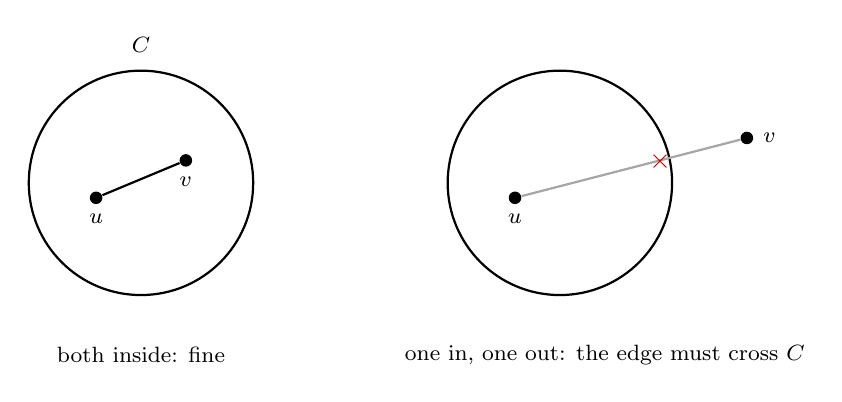
\begin{tikzpicture}[scale=0.95,
    vtx/.style={circle,fill=black,inner sep=1.6pt},
    every node/.style={font=\footnotesize}]
  % both endpoints inside
  \draw[thick] (0,0) circle (1.5);
  \node at (0,1.85) {$C$};
  \node[vtx,label=below:$u$] (u) at (-0.6,-0.2) {};
  \node[vtx,label=below:$v$] (v) at (0.6,0.3) {};
  \draw[thick] (u)--(v);
  \node at (0,-2.3) {both inside: fine};
  % one in, one out
  \begin{scope}[xshift=5.6cm]
    \draw[thick] (0,0) circle (1.5);
    \node[vtx,label=below:$u$] (u2) at (-0.6,-0.2) {};
    \node[vtx,label=right:$v$] (v2) at (2.5,0.6) {};
    \draw[thick,black!35] (u2)--(v2);
    \node[red!75!black,font=\bfseries] at (1.34,0.28) {$\times$};
    \node at (0.6,-2.3) {one in, one out: the edge must cross $C$};
  \end{scope}
\end{tikzpicture}
\caption{A cycle separates the plane: edges avoiding it cannot cross it.}
\label{fig:planar-jordan}
\end{figure}

So once we commit to drawing a cycle $C$, the rest of the graph decomposes into
chunks, and each chunk must be placed entirely inside or entirely outside. This
turns a continuous drawing problem into a discrete two-way choice --- and
two-way choices are exactly what $2$-colouring solves.

\subsection{Segments and interlacement}\label{sec:planar-segments}

The planarity test needs a vocabulary for the pieces of the graph that hang off
a cycle, and for when two such pieces get in each other's way.

\begin{definition}[Segment]\label{def:planar-segment}
Fix a cycle $C$ in $G$. A \emph{segment} (also called a \emph{bridge} of $C$)
is either
\begin{itemize}[nosep]
  \item an edge of $G$ joining two non-consecutive vertices of $C$ --- a
        \emph{chord}; or
  \item the subgraph induced by the edges of one connected component of
        $G - V(C)$, together with all edges joining that component to $C$.
\end{itemize}
The vertices of $C$ that a segment touches are its \emph{attachments}.
\end{definition}

By Observation~\ref{obs:planar-key}, each segment must be drawn entirely inside $C$ or
entirely outside $C$; it cannot be split, because it is connected and avoids
$C$ except at its attachments.

\begin{figure}[ht]
\centering
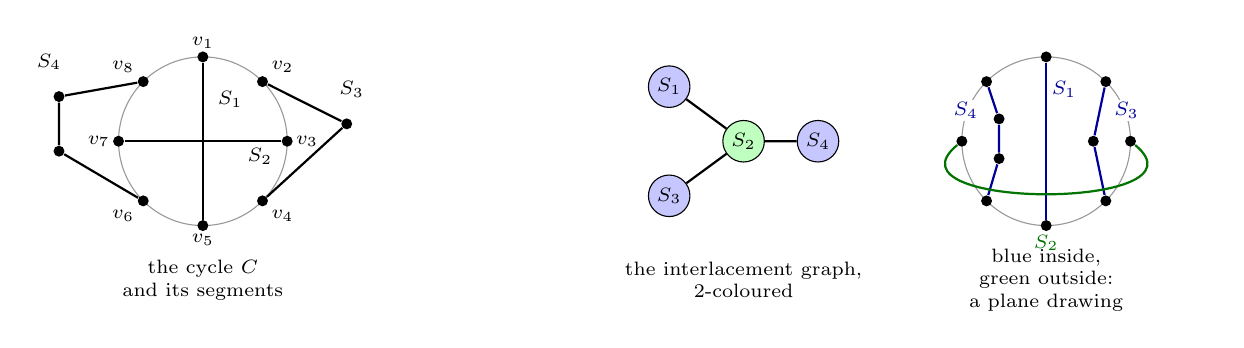
\begin{tikzpicture}[scale=0.63,
    vtx/.style={circle,fill=black,inner sep=1.4pt},
    sg/.style={circle,draw,fill=white,inner sep=1pt,minimum size=15pt,
               font=\scriptsize},
    ins/.style={blue!60!black,thick},
    outs/.style={green!45!black,thick},
    every node/.style={font=\scriptsize}]
  %-------------------------------------------------- panel 1: the segments
  \begin{scope}
    \draw[black!40] (0,0) circle (1.7);
    \foreach \i in {1,...,8}{
      \node[vtx,label={[label distance=-2.5pt]{135-45*\i}:$v_\i$}]
           (u\i) at ({135-45*\i}:1.7) {};
    }
    \draw[thick] (u1)--(u5);
    \draw[thick] (u3)--(u7);
    \node[vtx] (p) at (2.9,0.35) {};
    \draw[thick] (u2)--(p) (u4)--(p);
    \node[vtx] (q1) at (-2.9,-0.2) {};
    \node[vtx] (q2) at (-2.9,0.9) {};
    \draw[thick] (q1)--(q2) (u6)--(q1) (u8)--(q2);
    \node at (0.55,0.85) {$S_1$};
    \node at (1.15,-0.3) {$S_2$};
    \node at (3.0,1.05) {$S_3$};
    \node at (-3.1,1.6) {$S_4$};
    \node[align=center] at (0,-2.8) {the cycle $C$\\ and its segments};
  \end{scope}
  %-------------------------------------------------- panel 2: interlacement
  \begin{scope}[xshift=9.4cm]
    % the colours here are the ones panel 3 draws with: blue inside, green out
    \node[sg,fill=blue!22]  (t1) at (0,1.1)   {$S_1$};
    \node[sg,fill=green!25] (t2) at (1.5,0)   {$S_2$};
    \node[sg,fill=blue!22]  (t3) at (0,-1.1)  {$S_3$};
    \node[sg,fill=blue!22]  (t4) at (3.0,0)   {$S_4$};
    \draw[thick] (t1)--(t2) (t3)--(t2) (t4)--(t2);
    \node[align=center] at (1.5,-2.8)
      {the interlacement graph,\\ $2$-coloured};
  \end{scope}
  %-------------------------------------------------- panel 3: the drawing
  \begin{scope}[xshift=17.0cm]
    \draw[black!40] (0,0) circle (1.7);
    \foreach \i in {1,...,8}{
      \node[vtx] (w\i) at ({135-45*\i}:1.7) {};
    }
    \draw[ins] (w1)--(w5);
    \node[vtx] (r) at (0.95,0) {};
    \draw[ins] (w2)--(r) (w4)--(r);
    \node[vtx] (z1) at (-0.95,-0.35) {};
    \node[vtx] (z2) at (-0.95,0.45) {};
    \draw[ins] (z1)--(z2) (w6)--(z1) (w8)--(z2);
    \draw[outs] (w3) .. controls (3.4,-1.4) and (-3.4,-1.4) .. (w7);
    \node[blue!60!black,font=\scriptsize,fill=white,inner sep=1pt]
      at (0.36,1.05) {$S_1$};
    \node[green!45!black,font=\scriptsize,fill=white,inner sep=1pt]
      at (0,-2.05) {$S_2$};
    \node[blue!60!black,font=\scriptsize,fill=white,inner sep=1pt]
      at (1.62,0.62) {$S_3$};
    \node[blue!60!black,font=\scriptsize,fill=white,inner sep=1pt]
      at (-1.62,0.62) {$S_4$};
    \node[align=center,text width=2.9cm] at (0,-2.8)
      {blue inside, green outside:\\ a plane drawing};
  \end{scope}
\end{tikzpicture}
\caption{From a cycle to segments to the interlacement graph to a drawing.}
\label{fig:planar-segments}
\end{figure}

Now, when can two segments be placed on the same side? If their attachments
interleave around the cycle, they cannot: drawing both inside would force them
to cross.

\begin{definition}[Conflict / interlacement]\label{def:planar-interlace}
Two segments $S$ and $S'$ \emph{conflict} (or \emph{interlace}) if there are
four vertices $v_1,v_2,v_3,v_4$ occurring in this cyclic order on $C$ with
$v_1,v_3$ attachments of $S$ and $v_2,v_4$ attachments of $S'$.
The \emph{interlacement graph} $I$ has one vertex per segment, with an edge
between two segments exactly when they conflict.
\end{definition}

\begin{remark}[A case the slides gloss over]\label{rem:planar-threeattach}
There is a second way two segments can fail to share a side: if they have
\emph{three or more attachments in common}. Suppose $S$ and $S'$ both attach at
$a,b,c$. Drawing $S$ inside $C$ cuts the disc into three regions, each of whose
boundary contains only two of $a,b,c$; so $S'$, which must live in one region,
cannot reach all three. These pairs are not always caught by
Definition~\ref{def:planar-interlace} (the four witnesses would have to repeat a
vertex), so a correct implementation must add them to $I$ explicitly. This is
standard in the literature; see the optional Auslander--Parter reading in the
course archive.
\end{remark}

\begin{figure}[ht]
\centering
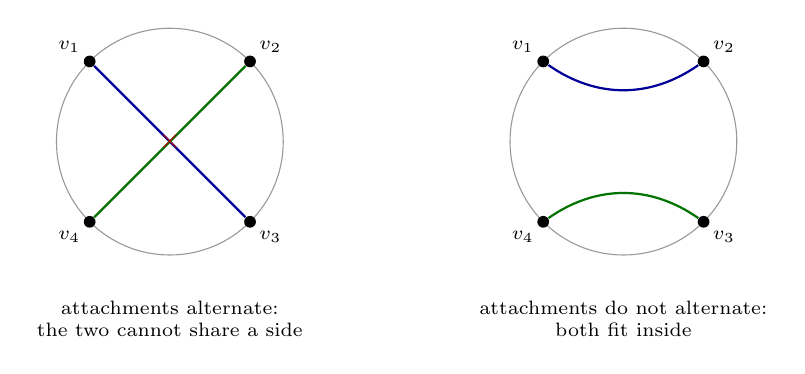
\begin{tikzpicture}[scale=0.9,
    vtx/.style={circle,fill=black,inner sep=1.5pt},
    sa/.style={blue!60!black,thick},
    sb/.style={green!45!black,thick},
    every node/.style={font=\scriptsize}]
  % interlacing
  \begin{scope}
    \draw[black!40] (0,0) circle (1.6);
    \foreach \i/\n in {1/{v_1}, 2/{v_2}, 3/{v_3}, 4/{v_4}}{
      \node[vtx,label={[label distance=-2.5pt]{135-90*\i+90}:$\n$}]
           (a\i) at ({135-90*\i+90}:1.6) {};
    }
    \draw[sa] (a1)--(a3);
    \draw[sb] (a2)--(a4);
    \node[red!75!black,font=\bfseries] at (0,0) {$\times$};
    \node[align=center] at (0,-2.5)
      {attachments alternate:\\ the two cannot share a side};
  \end{scope}
  % not interlacing
  \begin{scope}[xshift=6.4cm]
    \draw[black!40] (0,0) circle (1.6);
    \foreach \i/\n in {1/{v_1}, 2/{v_2}, 3/{v_3}, 4/{v_4}}{
      \node[vtx,label={[label distance=-2.5pt]{135-90*\i+90}:$\n$}]
           (b\i) at ({135-90*\i+90}:1.6) {};
    }
    \draw[sa] (b1) to[bend right=35] (b2);
    \draw[sb] (b3) to[bend right=35] (b4);
    \node[align=center] at (0,-2.5)
      {attachments do not alternate:\\ both fit inside};
  \end{scope}
\end{tikzpicture}
\caption{Interlacing segments cannot share a side.}
\label{fig:planar-interlace}
\end{figure}

\begin{observation}\label{obs:planar-2col}
If $G$ is planar, then in any plane embedding the segments placed inside $C$
form an independent set of $I$, as do those placed outside. Hence $I$ must be
$2$-colourable, i.e.\ bipartite.
\end{observation}

This gives us a necessary condition that we can test in linear time
($2$-colourability is a BFS). It is not by itself sufficient --- a segment
placed inside must also be drawable inside, which is a planarity question one
level down --- and that is what makes the algorithm recursive.

\subsection{The algorithm}

\begin{algorithm}[ht]
\caption{Planarity test (first attempt)}
\label{alg:planar-naive}
\begin{algorithmic}[1]
  \State find a cycle $C$ in $G$; let $S_1,\dots,S_k$ be its segments
  \If{the interlacement graph $I$ is not $2$-colourable}
    \State \Return NO
  \EndIf
  \For{$i = 1,\dots,k$}
    \State recursively test whether $C + S_i$ is planar
  \EndFor
  \State \Return YES iff all recursive calls returned YES
\end{algorithmic}
\end{algorithm}

Why is this the right recursion? Two directions.

\begin{itemize}
  \item \textbf{Soundness.} If $I$ is not $2$-colourable then $G$ is not planar
        by Observation~\ref{obs:planar-2col}. If some $C + S_i$ is not planar, then
        $G$ is not planar either, since $C + S_i$ is a subgraph of $G$.
  \item \textbf{Completeness.} Suppose $I$ is $2$-colourable and each
        $C + S_i$ is planar. Take a $2$-colouring of $I$; it tells us which
        segments go inside and which go outside. Each $C + S_i$ has a plane
        embedding, which we may take with $S_i$ drawn inside $C$ (if it is
        drawn outside, invert the drawing through a circle, or think of it on
        the sphere and rotate). Now merge: draw $C$ once, and for each $i$ paste
        in the drawing of $S_i$, on the side dictated by the colouring. Two
        segments on the same side do not conflict, so their attachments do not
        interleave and their drawings can be arranged in disjoint parts of the
        disc without crossings.
\end{itemize}

\begin{figure}[ht]
\centering
\begin{tikzpicture}[scale=0.8,
    vtx/.style={circle,fill=black,inner sep=1.3pt},
    ins/.style={blue!60!black,thick},
    outs/.style={green!45!black,thick},
    every node/.style={font=\scriptsize}]
  % three separately computed drawings, each with its segment inside
  \foreach \s/\dy/\col/\lbl in {a/2.4/{blue!60!black}/{$C+S_1$},
      b/0/{green!45!black}/{$C+S_2$}, c/-2.4/{green!45!black}/{$C+S_3$}}{
    \begin{scope}[yshift=\dy cm]
      \draw[black!40] (0,0) circle (0.95);
      \node[\col,font=\scriptsize] at (0,0) {$S$};
      \node[left=3pt] at (-0.95,0) {\lbl};
      \draw[-{Latex[length=2mm]},black!45] (1.2,0) -- (2.6,{-\dy*0.42});
    \end{scope}
  }
  % the merged drawing
  \begin{scope}[xshift=5.6cm]
    \draw[black!40] (0,0) circle (1.9);
    \foreach \i in {1,...,8}{ \node[vtx] (m\i) at ({135-45*\i}:1.9) {}; }
    \draw[ins] (m1) to[bend right=25] (m4);
    \node[blue!60!black,fill=white,inner sep=1pt] at (0.75,0.55) {$S_1$};
    \draw[outs] (m2) .. controls (3.6,1.6) and (3.6,-1.2) .. (m5);
    \node[green!45!black,fill=white,inner sep=1pt] at (3.05,0.35) {$S_2$};
    \draw[outs] (m6) .. controls (-3.4,-1.6) and (-3.4,1.2) .. (m8);
    \node[green!45!black,fill=white,inner sep=1pt] at (-2.95,-0.3) {$S_3$};
    \node[align=center] at (0,-2.9)
      {$C$ is drawn once; each segment is pasted\\
       on the side its colour dictates};
  \end{scope}
  \node[align=center] at (0,-4.3)
    {the pieces meet only on $C$};
\end{tikzpicture}
\caption{Merging the recursive drawings using the $2$-colouring.}
\label{fig:planar-merge}
\end{figure}

\subsection{The catch, and separating cycles}\label{sec:planar-sepcyclesec}

Algorithm~\ref{alg:planar-naive} has a bug, and it is a fatal one: the
recursion need not make progress. If $C$ happens to have only one segment
$S_1$, then $C + S_1 = G$, and we recurse on the very same graph forever.

The fix is to insist on a cycle that actually splits something off.

\begin{definition}
A cycle $C$ in $G$ is \emph{separating} if it has at least two segments.
\end{definition}

If $C$ is separating, then every $C + S_i$ is a proper subgraph of $G$ (it
misses at least the edges of the other segment), so the recursion strictly
descends. It remains to show that separating cycles exist, except in cases so
simple that we can answer directly.

\begin{lemma}[Existence of a separating cycle]\label{lem:planar-sepcycle}
Let $G$ be $2$-connected. Then $G$ has a separating cycle unless
\begin{enumerate}[label=(\roman*),nosep]
  \item $G$ is itself a cycle, or
  \item $G$ is a cycle plus one segment which is a path.
\end{enumerate}
Moreover, a separating cycle can be found in polynomial (indeed linear) time.
\end{lemma}

Both exceptional cases are trivially planar: (i) is a circle, and (ii) is a
\emph{theta graph}, drawn as a circle with one path across the inside. So the
lemma loses us nothing.

\begin{proof}
Find any cycle $C$ (one exists since $G$ is $2$-connected). If $C$ has at
least two segments we are done. If $C$ has no segments then $G = C$ and we are
in case~(i). So assume $C$ has exactly one segment $S$. If $S$ is a path, we
are in case~(ii). So assume $S$ is a single segment that is \emph{not} a path;
we construct a separating cycle.

Since $G$ is $2$-connected, $S$ has at least two attachments on $C$. Pick two
attachments $u$ and $v$ that are \emph{consecutive}, meaning that one of the
two $u$--$v$ arcs of $C$ contains no attachment of $S$ in its interior. Call
that arc $B$, and call the other arc $A$; so $A$ contains all the remaining
attachments of $S$, if any.

Because $S$ is connected and attaches at both $u$ and $v$, it contains a path
$P$ from $u$ to $v$ whose interior vertices lie entirely inside $S$ (in
particular, off $C$). Set
\[
  C' \;:=\; A + P ,
\]
which is a cycle: $A$ is a $u$--$v$ path along $C$, $P$ is a $u$--$v$ path
through $S$, and they meet only at $u$ and $v$.

We claim $C'$ is separating, i.e.\ that it has at least two segments.
\begin{itemize}[nosep]
  \item The arc $B$ gives one segment of $C'$: its interior vertices are off
        $C'$ and connect to $C'$ exactly at $u$ and $v$. (If $B$ has no
        interior vertices then $B$ is a single edge $uv$, which is a chord of
        $C'$ because $P$ has length at least $2$; either way, a segment.)
  \item Since $S$ is not a path, $S$ has at least one edge outside $P$. That
        edge is not on $C'$ either, so it belongs to some segment of $C'$, and
        that segment is different from the one contributed by $B$ --- it lives
        on the other side, attached to $A \cup P$ rather than only to
        $\{u,v\}$.
\end{itemize}
So $C'$ has at least two segments and is separating. All the steps ---
finding a cycle, finding attachments, finding $P$ --- are searches in a graph
and run in linear time.
\end{proof}

\begin{figure}[ht]
\centering
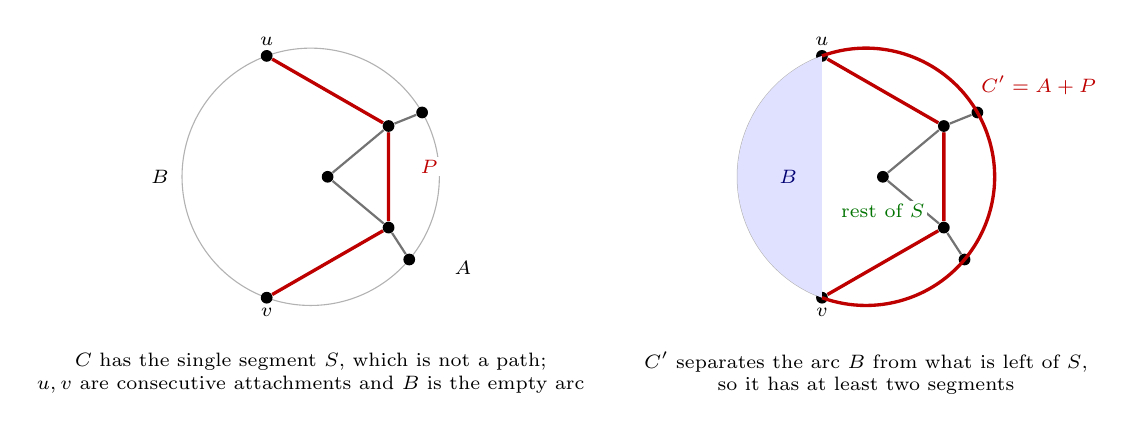
\begin{tikzpicture}[scale=0.86,
    vtx/.style={circle,fill=black,inner sep=1.5pt},
    seg/.style={black!55,thick},
    pth/.style={red!75!black,line width=1.2pt},
    every node/.style={font=\scriptsize}]
  \foreach \s/\dx in {a/0, b/8.2}{
    \begin{scope}[xshift=\dx cm]
      % the cycle C, with u and v consecutive attachments
      \draw[black!30] (0,0) circle (1.9);
      \node[vtx,label={[label distance=-2pt]above:$u$}] (u\s) at (110:1.9) {};
      \node[vtx,label={[label distance=-2pt]below:$v$}] (v\s) at (250:1.9) {};
      \node[vtx] (x\s) at (30:1.9) {};
      \node[vtx] (y\s) at (-40:1.9) {};
      % the segment S, drawn to the right
      \node[vtx] (s1\s) at (1.15,0.75) {};
      \node[vtx] (s2\s) at (1.15,-0.75) {};
      \node[vtx] (s3\s) at (0.25,0) {};
      \draw[seg] (u\s)--(s1\s) (s1\s)--(s2\s) (s2\s)--(v\s)
                 (s1\s)--(s3\s) (s3\s)--(s2\s) (s1\s)--(x\s) (s2\s)--(y\s);
    \end{scope}
  }
  % panel 1: label the arcs and the path
  \node[left] at (-1.95,0) {$B$};
  \node[right] at (1.98,-1.35) {$A$};
  \draw[pth] (ua)--(s1a)--(s2a)--(va);
  \node[red!75!black,fill=white,inner sep=1pt] at (1.75,0.15) {$P$};
  \node[align=center] at (0,-2.9)
    {$C$ has the single segment $S$, which is not a path;\\
     $u,v$ are consecutive attachments and $B$ is the empty arc};
  % panel 2: the new cycle
  \begin{scope}[xshift=8.2cm]
    \draw[pth] (ub) arc (110:-110:1.9);
    \draw[pth] (ub)--(s1b)--(s2b)--(vb);
    \node[red!75!black,fill=white,inner sep=1.5pt] at (2.55,1.35)
      {$C' = A + P$};
    \fill[blue!12] (110:1.9) arc (110:250:1.9) -- cycle;
    \node[blue!45!black] at (-1.15,0) {$B$};
    \node[green!45!black,fill=white,inner sep=1pt] at (0.25,-0.5)
      {rest of $S$};
    \node[align=center] at (0,-2.9)
      {$C'$ separates the arc $B$ from what is left of $S$,\\
       so it has at least two segments};
  \end{scope}
\end{tikzpicture}
\caption{Building a separating cycle $C' = A + P$ when $C$ has a single
non-path segment.}
\label{fig:planar-sepcycle}
\end{figure}

\begin{algorithm}[ht]
\caption{Planarity test (corrected)}
\label{alg:planar}
\begin{algorithmic}[1]
  \State reduce to the $2$-connected case; if $m > 3n-6$ \Return NO
  \If{$G$ is a cycle, or a cycle plus a path segment}
    \State \Return YES
  \EndIf
  \State find a \emph{separating} cycle $C$ (Lemma~\ref{lem:planar-sepcycle}); let
         $S_1,\dots,S_k$ be its segments
  \If{the interlacement graph $I$ is not $2$-colourable}
    \State \Return NO
  \EndIf
  \For{$i = 1,\dots,k$}
    \State recursively test whether $C + S_i$ is planar
  \EndFor
  \State \Return YES iff all recursive calls returned YES
\end{algorithmic}
\end{algorithm}

\subsection{Running time}

Each recursive call does a bounded amount of graph work: find a separating
cycle (linear), compute the segments (a connected-components computation,
linear), build the interlacement graph (at most $\bigoh{n^2}$, since there are
$\bigoh{n}$ segments and comparing two segments' attachment patterns takes
linear time), and $2$-colour it (linear in its size, $\bigoh{n^2}$). So a call
costs $\bigoh{n^2}$.

How many calls are there? Each call passes a strictly smaller graph
$C + S_i$ to its children, but the pieces overlap in $C$, so the naive bound
is not immediate.

\begin{quote}
\textbf{Fact (stated without proof).} The total number of recursive calls is
at most $m$. The argument charges each call to a distinct edge of $G$; the
details are omitted here.
\end{quote}

Since we may assume $m = \bigoh{n}$, we get $\bigoh{n}$ calls of cost
$\bigoh{n^2}$ each:
\[
  \text{total running time } \; \bigoh{n^3}.
\]

\begin{intuition}
Step back and look at the shape of this algorithm. It converts a
\emph{geometric} question --- can this be drawn? --- into a
\emph{combinatorial} one --- can these choices be made consistently? The
conversion happens in two moves. Observation~\ref{obs:planar-key} says the only choice
is binary (inside or outside). Definition~\ref{def:planar-interlace} records which
binary choices are incompatible. What is left is $2$-colouring, which is easy,
plus a recursion to check that each individual choice can actually be realised.

The one place where care is genuinely needed is the recursion measure, which is
also the one place where the naive version was simply wrong. That is a common
pattern: the interesting bug is never in the clever idea, it is in the
termination argument.
\end{intuition}

%==============================================================================
\section{The Planar Separator Theorem}\label{sec:planar-pst}
%==============================================================================

We now turn to the structural property that makes planar graphs
algorithmically soft: they can be cut into balanced pieces very cheaply.

\begin{definition}[Balanced separator]
Let $\alpha \in (0,1)$. A set $S \subseteq V$ is an
\emph{$\alpha$-balanced separator} of $G$ if every connected component of
$G - S$ has at most $\alpha \cdot n$ vertices.
\end{definition}

Note what is \emph{not} required: $G - S$ may have many components, and they
need not be balanced against each other. All we ask is that no single component
is large.

\begin{theorem}[Planar Separator Theorem]\label{thm:planar-pst}
Let $G = (V,E)$ be a planar graph on $n$ vertices. Then $G$ has a
$\tfrac{9}{10}$-balanced separator of size at most $11\sqrt{n}$.
Moreover, such a separator can be found in polynomial time.
\end{theorem}

Several proofs exist. The classical one is due to Lipton and Tarjan (1979),
who obtained a $\tfrac{2}{3}$-balanced separator of size $2\sqrt{2}\sqrt{n}$
using breadth-first search layers; it is combinatorial and constructive. The
proof sketched below is geometric and probabilistic, and it generalises better.
The exact constants are of no importance for us --- what matters is
$\bigoh{\sqrt n}$.

\begin{figure}[ht]
\centering
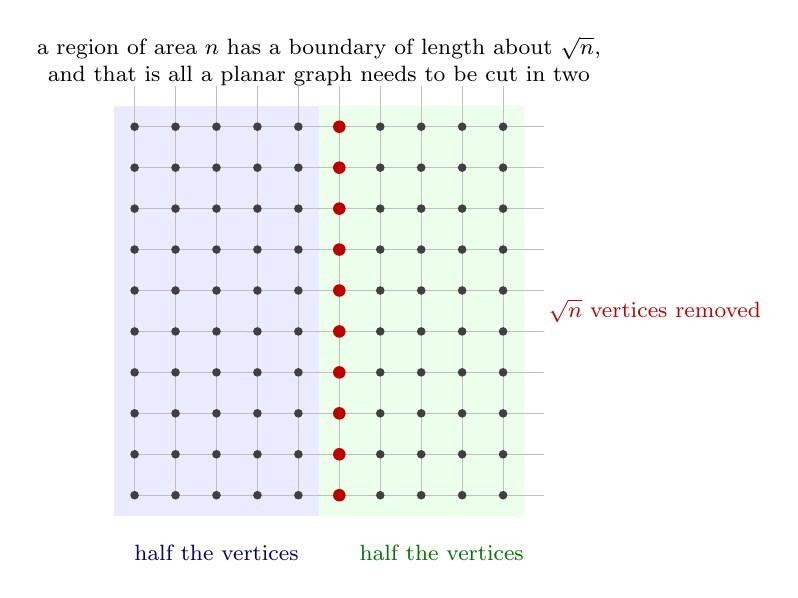
\begin{tikzpicture}[scale=0.52,
    sm/.style={circle,fill=black!75,inner sep=1.1pt},
    sep/.style={circle,fill=red!75!black,inner sep=1.6pt},
    every node/.style={font=\footnotesize}]
  \fill[blue!8]  (0.5,0.5) rectangle (5.5,10.5);
  \fill[green!8] (5.5,0.5) rectangle (10.5,10.5);
  \foreach \i in {1,...,10}{ \foreach \j in {1,...,10}{
    \draw[black!25] (\i,\j) -- ++(1,0);
    \draw[black!25] (\i,\j) -- ++(0,1);
  }}
  \foreach \i in {1,...,10}{ \foreach \j in {1,...,10}{
    \ifnum\i=6 \node[sep] at (\i,\j) {}; \else \node[sm] at (\i,\j) {}; \fi
  }}
  \node[blue!45!black] at (3,-0.4) {half the vertices};
  \node[green!45!black] at (8.5,-0.4) {half the vertices};
  \node[red!75!black,right=4pt] at (10.6,5.5) {$\bigoh{\sqrt n}$ vertices removed};
  \node[align=center] at (5.5,11.6)
    {a region of area $n$ has a boundary of length about $\sqrt n$,\\
     and that is all a planar graph needs to be cut in two};
\end{tikzpicture}
\caption{A balanced separator: remove $\bigoh{\sqrt n}$ vertices, and nothing
big survives.}
\label{fig:planar-separator}
\end{figure}

\subsection{The bound is tight}

A separator theorem is only as good as its size bound, so it is worth asking
whether $\bigoh{\sqrt n}$ can be improved. It cannot, and the grid is the
reason.

\begin{proposition}\label{prop:planar-gridtight}
The $\sqrt{n} \times \sqrt{n}$ grid has no $\tfrac{9}{10}$-balanced separator
of size $\sqrt{n}/20$.
\end{proposition}

So Theorem~\ref{thm:planar-pst} is optimal up to the constant factor, and no cleverer
argument will get us to, say, $\bigoh{n^{1/3}}$.

\begin{intuition}
The grid is the canonical hard case and it is worth carrying around as a mental
image. To break a $\sqrt n \times \sqrt n$ grid into pieces of at most
$\tfrac{9}{10}$ of the area you must cut it more or less all the way across,
and going all the way across costs about $\sqrt n$ vertices. Any set that is
too small leaves a ``highway'' of untouched rows and columns, and the untouched
part stays connected and large.

The same picture explains why $\sqrt{n}$ is the right exponent in general:
planar graphs are two-dimensional, and in two dimensions the boundary of a
region of area $A$ has length about $\sqrt{A}$. The Planar Separator Theorem
is the combinatorial shadow of the isoperimetric inequality.
\end{intuition}

\begin{figure}[ht]
\centering
\begin{tikzpicture}[scale=0.42,
    sm/.style={circle,fill=black!75,inner sep=1.0pt},
    del/.style={red!75!black,line width=0.8pt},
    sep/.style={circle,fill=red!75!black,inner sep=1.4pt},
    every node/.style={font=\footnotesize}]
  \foreach \s/\dx in {a/0, b/14}{
    \begin{scope}[xshift=\dx cm]
      \foreach \i in {1,...,10}{ \foreach \j in {1,...,10}{
        \draw[black!25] (\i,\j) -- ++(1,0);
        \draw[black!25] (\i,\j) -- ++(0,1);
      }}
    \end{scope}
  }
  % left: a scattered handful of deletions leaves everything connected
  \foreach \i in {1,...,10}{ \foreach \j in {1,...,10}{ \node[sm] at (\i,\j) {}; }}
  \foreach \c in {{3,7},{6,2},{8,9},{2,3},{9,5},{5,5}}{
    \draw[del] ($(\c)+(-0.28,-0.28)$) -- ++(0.56,0.56);
    \draw[del] ($(\c)+(-0.28,0.28)$) -- ++(0.56,-0.56);
  }
  \node[align=center] at (5.5,-1.4)
    {a handful of deletions:\\ whole rows and columns survive};
  % right: a full column really does separate
  \begin{scope}[xshift=14cm]
    \fill[blue!8]  (0.5,0.5) rectangle (5.5,10.5);
    \fill[green!8] (5.5,0.5) rectangle (10.5,10.5);
    \foreach \i in {1,...,10}{ \foreach \j in {1,...,10}{
      \ifnum\i=6 \node[sep] at (\i,\j) {}; \else \node[sm] at (\i,\j) {}; \fi
    }}
    \node[align=center] at (5.5,-1.4)
      {a full column, $\sqrt n$ vertices,\\ and not one fewer};
  \end{scope}
\end{tikzpicture}
\caption{Small sets cannot disconnect the grid.}
\label{fig:planar-gridtight}
\end{figure}

\subsection{Koebe's theorem and the proof idea (non-examinable)}
\label{sec:planar-koebe-nonexam}

The geometric proof rests on a beautiful and surprising representation
theorem.

\begin{theorem}[Koebe's disk embedding theorem]\label{thm:planar-koebe}
Every planar graph $G$ can be represented by a family of disks $\{D_v\}_{v \in
V}$ in the plane such that
\begin{enumerate}[label=(\roman*),nosep]
  \item the interiors of the disks are pairwise disjoint, and
  \item $D_v$ and $D_w$ touch if and only if $\{v,w\} \in E$.
\end{enumerate}
\end{theorem}

In other words, every planar graph \emph{is} a coin-contact graph. This
converts a combinatorial object into a rigid geometric one, at which point
geometric tools --- areas, random circles --- become available.

\begin{figure}[ht]
\centering
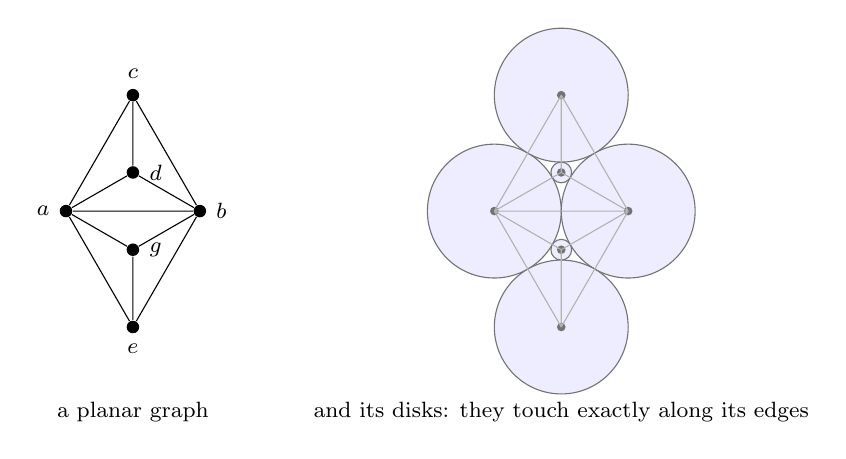
\begin{tikzpicture}[scale=0.85,
    vtx/.style={circle,fill=black,inner sep=1.6pt},
    dsk/.style={draw=black!55,fill=blue!7},
    every node/.style={font=\footnotesize}]
  % the graph
  \begin{scope}
    \node[vtx,label=left:$a$]  (a) at (0,0) {};
    \node[vtx,label=right:$b$] (b) at (2,0) {};
    \node[vtx,label=above:$c$] (c) at (1,1.732) {};
    \node[vtx,label=right:$d$] (d) at (1,0.577) {};
    \node[vtx,label=below:$e$] (e) at (1,-1.732) {};
    \node[vtx,label=right:$g$] (g) at (1,-0.577) {};
    \draw (a)--(b) (a)--(c) (b)--(c) (a)--(d) (b)--(d) (c)--(d)
          (a)--(e) (b)--(e) (a)--(g) (b)--(g) (e)--(g);
    \node at (1,-3.0) {a planar graph};
  \end{scope}
  % the packing
  \begin{scope}[xshift=6.4cm]
    \draw[dsk] (0,0) circle (1);
    \draw[dsk] (2,0) circle (1);
    \draw[dsk] (1,1.732) circle (1);
    \draw[dsk] (1,-1.732) circle (1);
    \draw[dsk] (1,0.5774) circle (0.1547);
    \draw[dsk] (1,-0.5774) circle (0.1547);
    \foreach \c in {{0,0},{2,0},{1,1.732},{1,-1.732},{1,0.5774},{1,-0.5774}}{
      \node[vtx,black!55,inner sep=1.1pt] at (\c) {};
    }
    \draw[black!30] (0,0)--(2,0) (0,0)--(1,1.732) (2,0)--(1,1.732)
      (0,0)--(1,0.5774) (2,0)--(1,0.5774) (1,1.732)--(1,0.5774)
      (0,0)--(1,-1.732) (2,0)--(1,-1.732) (0,0)--(1,-0.5774)
      (2,0)--(1,-0.5774) (1,-1.732)--(1,-0.5774);
    \node at (1,-3.0) {and its disks: they touch exactly along its edges};
  \end{scope}
\end{tikzpicture}
\caption{Koebe: every planar graph is the contact graph of a family of disks.}
\label{fig:planar-koebe}
\end{figure}

\begin{proof}[Sketch, for Theorem~\ref{thm:planar-pst}]
\nonexam{This proof goes beyond what is covered in the lecture. The statement
of the separator theorem is examinable; this sketch of why it is true is not.}
Fix a disk representation of $G$ as given by Theorem~\ref{thm:planar-koebe}.

Let $D$ be the smallest circle containing at least $n/10$ of the disk centres.
Rescale and translate so that $D$ has radius $1$ and is centred at the origin.
Pick $r \in [1,2]$ uniformly at random, let $C_r$ be the circle of radius $r$
about the origin, and set
\[
  S \;=\; \{\, v : D_v \text{ intersects } C_r \,\} ,
\]
a random set. Take $S$ as the separator; the vertices whose disks lie strictly
inside $C_r$ and those strictly outside form the two sides.

\emph{Why $S$ separates.} Two disks that do not meet $C_r$ and lie on opposite
sides of it cannot touch, so there is no edge between the inside part and the
outside part. This is the same Jordan-curve reasoning as
Observation~\ref{obs:planar-key}, now applied to a circle drawn through the packing.

\emph{Why $S$ is balanced.} The inside contains at least the $n/10$ centres
inside $D$. For the outside, one shows that the disk of radius $2$ cannot
contain too many centres: by minimality of $D$, every circle of radius smaller
than $1$ contains fewer than $n/10$ centres, and a disk of radius $2$ can be
covered by a constant number of such circles. Choosing the constants
appropriately gives that neither side exceeds $\tfrac{9}{10}n$.

\emph{Why $S$ is small.} This is the pretty part. A disk $D_v$ of radius $\rho_v$
meets $C_r$ only if $r$ falls in an interval of length about $2\rho_v$, so
\[
  \Pr[\,v \in S\,] \;\lesssim\; 2\rho_v ,
\]
because $r$ is uniform on an interval of length $1$. Hence
$\mathbb{E}[|S|] \lesssim 2\sum_v \rho_v$, where the sum ranges over the disks
that could possibly be hit --- essentially those inside the disk of radius
$2$ (only $\bigoh{1}$ disks are large enough to reach it from outside). Those
disks are interior-disjoint and fit inside a bounded region, so
$\sum_v \pi\rho_v^2 = \bigoh{1}$, and by Cauchy--Schwarz
\[
  \sum_{v} \rho_v \;\le\; \sqrt{ n \cdot \sum_v \rho_v^2 } \;=\; \bigoh{\sqrt n} .
\]
So $\mathbb{E}[|S|] = \bigoh{\sqrt{n}}$, and some choice of $r$ achieves the
expectation. Working out the constants carefully gives the $11\sqrt n$ of
Theorem~\ref{thm:planar-pst}.
\end{proof}

\begin{figure}[ht]
\centering
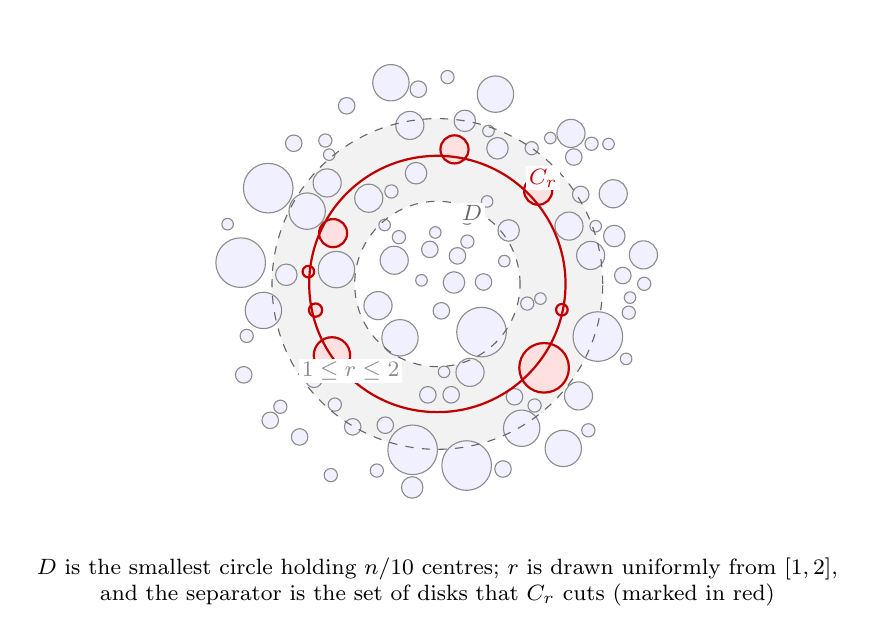
\begin{tikzpicture}[scale=1.05,
    dsk/.style={draw=black!45,fill=blue!6},
    cut/.style={draw=red!75!black,thick,fill=red!12},
    every node/.style={font=\footnotesize}]
  \begin{scope}
    \clip (-3.1,-3.1) rectangle (3.1,3.1);
    \fill[black!5,even odd rule] (0,0) circle (2) (0,0) circle (1);
    \draw[dsk] (-0.192,0.044) circle (0.070);
    \draw[dsk] (-1.737,1.702) circle (0.100);
    \draw[dsk] (0.727,1.641) circle (0.130);
    \draw[dsk] (-0.299,-2.006) circle (0.300);
    \draw[dsk] (1.734,1.083) circle (0.100);
    \draw[dsk] (0.534,-0.582) circle (0.300);
    \draw[dsk] (0.862,0.647) circle (0.130);
    \draw[dsk] (-0.333,1.918) circle (0.170);
    \draw[dsk] (-1.492,-1.153) circle (0.100);
    \draw[dsk] (-0.522,0.287) circle (0.170);
    \draw[dsk] (0.354,-2.196) circle (0.300);
    \draw[dsk] (1.941,-0.636) circle (0.300);
    \draw[dsk] (-1.289,-2.312) circle (0.080);
    \draw[dsk] (-2.046,1.159) circle (0.300);
    \draw[dsk] (1.020,-1.745) circle (0.220);
    \draw[dsk] (-0.452,-0.651) circle (0.220);
    \draw[dsk] (-1.097,2.155) circle (0.100);
    \draw[dsk] (0.794,-2.238) circle (0.100);
    \draw[dsk] (0.618,1.850) circle (0.070);
    \draw[dsk] (-0.718,-0.262) circle (0.170);
    \draw[dsk] (-0.091,0.418) circle (0.100);
    \draw[dsk] (-0.638,0.713) circle (0.070);
    \draw[dsk] (2.140,0.580) circle (0.130);
    \draw[dsk] (0.332,1.973) circle (0.130);
    \draw[dsk] (-0.304,-2.461) circle (0.130);
    \draw[dsk] (-1.221,0.174) circle (0.220);
    \draw[dsk] (0.123,2.502) circle (0.080);
    \draw[cut] (1.291,-1.014) circle (0.300);
    \draw[dsk] (-2.379,0.258) circle (0.300);
    \draw[dsk] (1.141,1.642) circle (0.080);
    \draw[dsk] (-0.830,1.037) circle (0.170);
    \draw[dsk] (1.087,-0.237) circle (0.080);
    \draw[dsk] (0.081,-1.063) circle (0.070);
    \draw[dsk] (-1.666,-1.850) circle (0.100);
    \draw[dsk] (1.915,0.699) circle (0.070);
    \draw[dsk] (0.602,0.998) circle (0.070);
    \draw[dsk] (0.395,-1.069) circle (0.170);
    \draw[dsk] (0.359,0.790) circle (0.070);
    \draw[dsk] (-1.308,1.564) circle (0.070);
    \draw[dsk] (-2.537,0.723) circle (0.070);
    \draw[cut] (-1.275,-0.864) circle (0.220);
    \draw[dsk] (2.502,0.002) circle (0.080);
    \draw[dsk] (0.703,2.296) circle (0.220);
    \draw[cut] (0.207,1.628) circle (0.170);
    \draw[dsk] (-1.333,1.222) circle (0.170);
    \draw[dsk] (2.330,-0.165) circle (0.070);
    \draw[dsk] (2.243,0.102) circle (0.100);
    \draw[cut] (-1.560,0.149) circle (0.070);
    \draw[dsk] (1.854,0.345) circle (0.170);
    \draw[dsk] (0.201,0.018) circle (0.130);
    \draw[dsk] (-0.230,2.356) circle (0.100);
    \draw[dsk] (-1.024,-1.728) circle (0.100);
    \draw[cut] (1.219,1.128) circle (0.170);
    \draw[dsk] (-2.306,-0.628) circle (0.080);
    \draw[dsk] (1.865,1.696) circle (0.080);
    \draw[dsk] (-0.258,1.340) circle (0.130);
    \draw[dsk] (0.558,0.024) circle (0.100);
    \draw[dsk] (1.707,-1.354) circle (0.170);
    \draw[dsk] (2.127,1.091) circle (0.170);
    \draw[cut] (-1.473,-0.316) circle (0.080);
    \draw[dsk] (0.810,0.277) circle (0.070);
    \draw[dsk] (-0.025,0.623) circle (0.070);
    \draw[dsk] (1.247,-0.177) circle (0.070);
    \draw[dsk] (-2.104,-0.320) circle (0.220);
    \draw[dsk] (-0.465,0.566) circle (0.080);
    \draw[dsk] (1.366,1.765) circle (0.070);
    \draw[dsk] (1.592,0.700) circle (0.170);
    \draw[cut] (-1.261,0.615) circle (0.170);
    \draw[dsk] (0.363,0.513) circle (0.080);
    \draw[dsk] (-1.240,-1.459) circle (0.080);
    \draw[dsk] (-1.899,-1.485) circle (0.080);
    \draw[dsk] (2.070,1.693) circle (0.070);
    \draw[cut] (1.506,-0.312) circle (0.070);
    \draw[dsk] (-1.355,1.735) circle (0.080);
    \draw[dsk] (1.826,-1.770) circle (0.080);
    \draw[dsk] (-0.732,-2.257) circle (0.080);
    \draw[dsk] (-2.342,-1.099) circle (0.100);
    \draw[dsk] (-1.575,0.881) circle (0.220);
    \draw[dsk] (2.315,-0.347) circle (0.080);
    \draw[dsk] (-0.562,2.434) circle (0.220);
    \draw[dsk] (-0.630,-1.708) circle (0.100);
    \draw[dsk] (2.283,-0.906) circle (0.070);
    \draw[dsk] (0.048,-0.325) circle (0.100);
    \draw[dsk] (-0.115,-1.341) circle (0.100);
    \draw[dsk] (1.650,1.535) circle (0.100);
    \draw[dsk] (1.523,-1.989) circle (0.220);
    \draw[dsk] (1.176,-1.470) circle (0.080);
    \draw[dsk] (0.933,-1.364) circle (0.100);
    \draw[dsk] (2.492,0.352) circle (0.170);
    \draw[dsk] (-2.021,-1.649) circle (0.100);
    \draw[dsk] (-0.556,1.119) circle (0.080);
    \draw[dsk] (0.167,-1.340) circle (0.100);
    \draw[dsk] (1.616,1.821) circle (0.170);
    \draw[dsk] (0.243,0.340) circle (0.100);
    \draw[dsk] (-1.827,0.111) circle (0.130);
  \end{scope}
  \draw[black!60,dashed] (0,0) circle (1);
  \draw[black!60,dashed] (0,0) circle (2);
  \draw[red!75!black,thick] (0,0) circle (1.55);
  \node[black!60,fill=white,inner sep=1pt] at (0.42,0.86) {$D$};
  \node[red!75!black,fill=white,inner sep=1pt] at (1.28,1.28) {$C_r$};
  \node[black!45,fill=white,inner sep=1pt] at (-1.05,-1.05) {$1 \le r \le 2$};
  \node[align=center] at (0,-3.6)
    {$D$ is the smallest circle holding $n/10$ centres; $r$ is drawn uniformly
     from $[1,2]$,\\ and the separator is the set of disks that $C_r$ cuts
     (marked in red)};
\end{tikzpicture}
\caption{A random circle in the annulus cuts few disks and splits the rest
evenly.}
\label{fig:planar-pst-proof}
\end{figure}

\begin{intuition}
The two requirements on $S$ pull in opposite directions, and the randomness is
what reconciles them. A circle far out is likely to cut few disks but leaves an
unbalanced split; a circle close in balances well but may slice through a lot.
Averaging over a whole range of radii shows that a good compromise must exist,
without ever having to point at it. This is the probabilistic method in its
purest form: we prove a separator exists by computing an average, and we never
construct one by hand.
\end{intuition}

%==============================================================================
\section{Application: independent set in \texorpdfstring{$2^{\bigoh{\sqrt n}}$}{2 to the O(sqrt n)} time}\label{sec:planar-mis}
%==============================================================================

\textsc{Maximum Independent Set} is NP-hard, and it stays NP-hard on planar
graphs. So we should not hope for a polynomial algorithm. But the separator
theorem buys us an enormous speed-up over the trivial $2^n$.

\begin{theorem}\label{thm:planar-mis}
\textsc{Maximum Independent Set} on planar graphs can be solved in
$2^{\bigoh{\sqrt n}}$ time.
\end{theorem}

\begin{intuition}
The idea is guess-and-divide. If we knew which separator vertices the optimal
solution uses, the problem would fall apart into independent subproblems, one
per component of $G - S$ --- because there are no edges between different
components, so their choices cannot interfere. We do not know, so we try all
possibilities. There are only $2^{|S|} = 2^{\bigoh{\sqrt n}}$ of them, which is
affordable, and each guess leaves subproblems that are a constant factor
smaller. The recursion depth is $\bigoh{\log n}$ and the sizes shrink
geometrically, so the $\sqrt{n}$ in the exponent survives to the end.
\end{intuition}

\begin{algorithm}[ht]
\caption{$\MIS(G)$ for planar $G$}
\label{alg:planar-mis}
\begin{algorithmic}[1]
  \If{$n$ is below a fixed constant} \Return a maximum independent set by
      brute force \EndIf
  \State find a $\tfrac{9}{10}$-balanced separator $S$ with
         $|S| \le 11\sqrt{n}$ \Comment{Theorem~\ref{thm:planar-pst}}
  \State let $G_1,\dots,G_t$ be the connected components of $G - S$
  \State $X \gets \emptyset$
  \ForAll{independent sets $I$ of $G[S]$}
    \For{$i = 1,\dots,t$}
      \State $I_i \gets \MIS\bigl(G_i - N(I)\bigr)$
    \EndFor
    \State $Y \gets I \cup I_1 \cup \dots \cup I_t$
    \If{$|Y| > |X|$} $X \gets Y$ \EndIf
  \EndFor
  \State \Return $X$
\end{algorithmic}
\end{algorithm}

\begin{figure}[ht]
\centering
\begin{tikzpicture}[scale=0.95,
    sv/.style={circle,fill=black,inner sep=1.6pt},
    ch/.style={circle,draw=red!75!black,thick,minimum size=11pt,inner sep=0pt},
    every node/.style={font=\footnotesize}]
  % the separator band
  \fill[red!8,rounded corners=8pt] (-0.45,-2.6) rectangle (0.45,2.6);
  \foreach \i/\y in {1/2.0, 2/1.0, 3/0.0, 4/-1.0, 5/-2.0}{
    \node[sv] (s\i) at (0,\y) {};
  }
  \node[red!75!black,above] at (0,2.7) {$S$, \ $|S| \le 11\sqrt n$};
  \node[ch] at (s1) {};
  \node[ch] at (s4) {};
  \node[red!75!black,left=8pt] at (s1) {$I$};
  % the two sides
  \foreach \s/\dx/\lbl in {a/-2.9/{$G_1$}, b/2.9/{$G_2$}}{
    \draw[black!45,fill=black!4] (\dx,0) ellipse (2.0 and 2.4);
    \node[black!55] at (\dx,2.0) {\lbl};
  }
  \foreach \p in {{-3.6,1.2},{-2.4,0.9},{-3.1,-0.2},{-2.0,-1.2},{-3.7,-1.4}}{
    \node[sv] at (\p) {};
  }
  \foreach \p in {{3.6,1.2},{2.4,0.9},{3.1,-0.2},{2.0,-1.2},{3.7,-1.4}}{
    \node[sv] at (\p) {};
  }
  % the neighbours of I, struck out
  \foreach \p in {{-2.4,0.9},{2.4,0.9},{2.0,-1.2}}{
    \draw[red!75!black] ($(\p)+(-0.16,-0.16)$) -- ++(0.32,0.32);
    \draw[red!75!black] ($(\p)+(-0.16,0.16)$) -- ++(0.32,-0.32);
  }
  \draw[black!45] (s1)--(-2.4,0.9) (s1)--(2.4,0.9) (s4)--(2.0,-1.2);
  \node[align=center] at (0,-3.4)
    {guess $I \subseteq S$; delete $N(I)$; recurse on each side, which is
     planar\\ and has at most $\tfrac{9}{10}n$ vertices};
\end{tikzpicture}
\caption{Guess the solution's trace on the separator; the rest decomposes.}
\label{fig:planar-mis}
\end{figure}

\begin{proof}[Correctness]
Let $O$ be a maximum independent set of $G$ and let $I^\star = O \cap S$. Since
$O$ is independent, so is $I^\star$ in $G[S]$; therefore $I^\star$ is one of the
sets enumerated in the loop. Consider that iteration.

No vertex of $O \setminus S$ is adjacent to a vertex of $I^\star$, so
$O \setminus S$ avoids $N(I^\star)$ entirely, hence
$O \cap V(G_i)$ is an independent set of $G_i - N(I^\star)$ for each $i$. By
induction the recursive call returns a maximum one, so
$|I_i| \ge |O \cap V(G_i)|$. Summing,
\[
  |Y| = |I^\star| + \sum_{i=1}^{t} |I_i|
      \;\ge\; |O \cap S| + \sum_{i=1}^{t} |O \cap V(G_i)| = |O| .
\]

Conversely every $Y$ constructed by the algorithm really is independent: $I$ is
independent by the choice of the loop; each $I_i$ is independent; there are no
edges between different components $G_i, G_j$; and there are no edges between
$I$ and any $I_i$ because we deleted $N(I)$ before recursing. So the algorithm
outputs an independent set of size at least $|O|$, i.e.\ a maximum one.

Finally, each subproblem $G_i - N(I)$ is an induced subgraph of a planar graph
and hence planar, so the recursion stays inside the class and the separator
theorem remains applicable.
\end{proof}

\begin{proof}[Running time]
Let $T(n)$ bound the running time on planar graphs with $n$ vertices. There are
at most $2^{|S|} \le 2^{11\sqrt{n}}$ candidate sets $I$; the components number
$t \le n$ and each has at most $\tfrac{9}{10}n$ vertices, so each recursive
call is on an instance of size at most $\tfrac{9}{10}n$. Absorbing the
polynomial work (finding the separator, computing components) into the
constants,
\[
  T(n) \;\le\; 2^{11\sqrt{n}} \cdot n \cdot T\!\left(\tfrac{9}{10}n\right)
  \;+\; \mathrm{poly}(n).
\]
We claim $T(n) \le 2^{1000\sqrt{n}}$ for all sufficiently large $n$. Inductively,
\[
  T(n) \;\le\; 2^{11\sqrt n}\cdot n\cdot 2^{1000\sqrt{9n/10}}
   \;=\; n \cdot 2^{\left(11 + 1000\sqrt{9/10}\right)\sqrt n}
   \;\le\; n \cdot 2^{959.7\sqrt{n}}
   \;\le\; 2^{1000\sqrt n},
\]
where the last step holds because $n \le 2^{40\sqrt n}$ for every $n \ge 1$.
For the base case, brute force costs $2^n \le 2^{1000\sqrt n}$ whenever
$n \le 10^6$, which covers all small instances comfortably.
\end{proof}

\begin{remark}
The constant $1000$ is absurd and is an artefact of the crude bookkeeping; the
point is only that \emph{some} constant works, giving
$2^{\bigoh{\sqrt n}}$. The same template --- separator, guess its trace,
recurse --- gives $2^{\bigoh{\sqrt n}}$ algorithms for a whole family of
problems on planar graphs, and it is one of the standard reasons to care about
Theorem~\ref{thm:planar-pst}. Note also that this is not merely a speed-up but a
qualitative change: under the Exponential Time Hypothesis, $2^{o(\sqrt n)}$ is
impossible for these problems, so $\sqrt n$ in the exponent is the truth.
\end{remark}

%==============================================================================
\section{What stays hard on planar graphs}\label{sec:planar-hardness}
%==============================================================================

Given Section~\ref{sec:planar-mis}, it is natural to hope that planarity tames NP-hard
problems in general. It does not. \emph{Most} NP-hard graph problems remain
NP-hard when the input is restricted to planar graphs --- including independent
set, vertex cover, dominating set, Hamiltonian cycle, and $3$-colouring. What
we gain is better exponential algorithms, not polynomial ones.

There are a few notable exceptions, and one of them is a pleasant surprise.

\subsection{Planar Clique is easy}

One pleasant consequence of the edge bound: a problem that is
\textrm{NP}-hard in general collapses on planar graphs, for a reason that takes
two lines.

\begin{probdef}{Planar Clique}
  \instance A planar graph $G$ and an integer $k$.
  \question Does $G$ contain a clique of size at least $k$?
\end{probdef}

\begin{proposition}
\textsc{Planar Clique} is solvable in polynomial time.
\end{proposition}

\begin{proof}
A clique of size $5$ is a $K_5$ subgraph, hence a $K_5$ minor, which is
impossible in a planar graph by Corollary~\ref{cor:planar-k5} and
Observation~\ref{obs:planar-minor-closed}. So every planar graph has clique number at
most $4$. Therefore: if $k \ge 5$, answer NO immediately; otherwise
$k \le 4$ and we can simply test all $\binom{n}{k} \le \binom{n}{4} =
\bigoh{n^4}$ subsets of size $k$.
\end{proof}

The moral is worth stating: the problem is not easy because we found a clever
algorithm, but because the structure theory forbids the interesting instances
from existing at all. When a restriction makes an NP-hard problem polynomial,
it is very often for this kind of reason.

\subsection{Planar 3-Colouring is NP-hard}\label{sec:planar-3col}

Now the other direction, as a sampler of how planar hardness proofs go.

\begin{probdef}{(Planar) 3-Coloring}
  \instance A (planar) graph $G$.
  \question Does $G$ have a $3$-colouring?
\end{probdef}

We reduce from general $\ThreeCol$, which is NP-hard. The difficulty is
obvious: a general graph need not be planar, and we must somehow simulate the
crossings. The tool is a \emph{crossover gadget}, a small planar graph that
lets two ``wires'' pass each other while preserving the colour each carries.

\begin{claim}[The crossover gadget]\label{claim:planar-gadget}
There is a planar graph $W$ with four distinguished corner vertices
$a, a', b, b'$ (drawn on the outer face, with $a$ opposite $a'$ and $b$
opposite $b'$) such that:
\begin{enumerate}[label=(\alph*),nosep]
  \item in \emph{any} $3$-colouring of $W$, opposite corners get the same
        colour, i.e.\ $c(a) = c(a')$ and $c(b) = c(b')$; and
  \item \emph{any} assignment of colours to the four corners in which opposite
        corners agree extends to a $3$-colouring of all of $W$.
\end{enumerate}
\end{claim}

The verification is a finite case check, and a small one. $W$ has exactly
twelve proper $3$-colourings, and permuting the three colours acts on them with
two orbits of six: one orbit gives all four corners the same colour, the other
gives $a,a'$ one colour and $b,b'$ another. \Cref{fig:planar-gadget} shows one
colouring from each orbit. Both parts of the claim can be read off that
statement --- every one of the twelve has $c(a) = c(a')$ and $c(b) = c(b')$,
which is (a); and the twelve realise all nine ways of choosing a colour for
$\{a,a'\}$ and a colour for $\{b,b'\}$, which is (b).

\begin{figure}[ht]
\centering
\begin{tikzpicture}[scale=1.0,
    ed/.style={black!70},
    cv/.style={circle,draw=black!75,minimum size=15pt,inner sep=0pt,
               font=\scriptsize},
    c1/.style={cv,fill=red!25},
    c2/.style={cv,fill=green!30!white},
    c3/.style={cv,fill=blue!20},
    trm/.style={font=\footnotesize,inner sep=1pt},
    every node/.style={font=\scriptsize}]
  \begin{scope}
    \coordinate (nL) at (0.00,2.70);
    \coordinate (wL) at (-2.70,0.00);
    \coordinate (eL) at (2.70,0.00);
    \coordinate (sL) at (0.00,-2.70);
    \coordinate (aL) at (-1.35,1.35);
    \coordinate (bL) at (0.00,1.35);
    \coordinate (cL) at (1.35,1.35);
    \coordinate (dL) at (-1.35,0.00);
    \coordinate (xL) at (0.00,0.00);
    \coordinate (fL) at (1.35,0.00);
    \coordinate (gL) at (-1.35,-1.35);
    \coordinate (hL) at (0.00,-1.35);
    \coordinate (iL) at (1.35,-1.35);
    \draw[ed] (nL) -- (aL);
    \draw[ed] (aL) -- (wL);
    \draw[ed] (wL) -- (gL);
    \draw[ed] (gL) -- (sL);
    \draw[ed] (sL) -- (iL);
    \draw[ed] (iL) -- (eL);
    \draw[ed] (eL) -- (cL);
    \draw[ed] (cL) -- (nL);
    \draw[ed] (nL) -- (bL);
    \draw[ed] (wL) -- (dL);
    \draw[ed] (eL) -- (fL);
    \draw[ed] (sL) -- (hL);
    \draw[ed] (aL) -- (bL);
    \draw[ed] (hL) -- (iL);
    \draw[ed] (dL) -- (gL);
    \draw[ed] (cL) -- (fL);
    \draw[ed] (xL) -- (bL);
    \draw[ed] (xL) -- (dL);
    \draw[ed] (xL) -- (fL);
    \draw[ed] (xL) -- (hL);
    \draw[ed] (bL) -- (dL);
    \draw[ed] (bL) -- (fL);
    \draw[ed] (hL) -- (dL);
    \draw[ed] (hL) -- (fL);
    \node[c1] (vnL) at (nL) {1};
    \node[c1] (vwL) at (wL) {1};
    \node[c1] (veL) at (eL) {1};
    \node[c1] (vsL) at (sL) {1};
    \node[c3] (vaL) at (aL) {3};
    \node[c2] (vbL) at (bL) {2};
    \node[c2] (vcL) at (cL) {2};
    \node[c3] (vdL) at (dL) {3};
    \node[c1] (vxL) at (xL) {1};
    \node[c3] (vfL) at (fL) {3};
    \node[c2] (vgL) at (gL) {2};
    \node[c2] (vhL) at (hL) {2};
    \node[c3] (viL) at (iL) {3};
    \node[trm,above=1pt of vnL] {$b$};
    \node[trm,left=1pt of vwL] {$a$};
    \node[trm,right=1pt of veL] {$a'$};
    \node[trm,below=1pt of vsL] {$b'$};
    \node[align=center,text width=5cm] at (0,-3.90) {all four corners take\\ the same colour};
  \end{scope}
  \begin{scope}[xshift=6.9cm]
    \coordinate (nR) at (0.00,2.70);
    \coordinate (wR) at (-2.70,0.00);
    \coordinate (eR) at (2.70,0.00);
    \coordinate (sR) at (0.00,-2.70);
    \coordinate (aR) at (-1.35,1.35);
    \coordinate (bR) at (0.00,1.35);
    \coordinate (cR) at (1.35,1.35);
    \coordinate (dR) at (-1.35,0.00);
    \coordinate (xR) at (0.00,0.00);
    \coordinate (fR) at (1.35,0.00);
    \coordinate (gR) at (-1.35,-1.35);
    \coordinate (hR) at (0.00,-1.35);
    \coordinate (iR) at (1.35,-1.35);
    \draw[ed] (nR) -- (aR);
    \draw[ed] (aR) -- (wR);
    \draw[ed] (wR) -- (gR);
    \draw[ed] (gR) -- (sR);
    \draw[ed] (sR) -- (iR);
    \draw[ed] (iR) -- (eR);
    \draw[ed] (eR) -- (cR);
    \draw[ed] (cR) -- (nR);
    \draw[ed] (nR) -- (bR);
    \draw[ed] (wR) -- (dR);
    \draw[ed] (eR) -- (fR);
    \draw[ed] (sR) -- (hR);
    \draw[ed] (aR) -- (bR);
    \draw[ed] (hR) -- (iR);
    \draw[ed] (dR) -- (gR);
    \draw[ed] (cR) -- (fR);
    \draw[ed] (xR) -- (bR);
    \draw[ed] (xR) -- (dR);
    \draw[ed] (xR) -- (fR);
    \draw[ed] (xR) -- (hR);
    \draw[ed] (bR) -- (dR);
    \draw[ed] (bR) -- (fR);
    \draw[ed] (hR) -- (dR);
    \draw[ed] (hR) -- (fR);
    \node[c3] (vnR) at (nR) {3};
    \node[c2] (vwR) at (wR) {2};
    \node[c2] (veR) at (eR) {2};
    \node[c3] (vsR) at (sR) {3};
    \node[c1] (vaR) at (aR) {1};
    \node[c2] (vbR) at (bR) {2};
    \node[c1] (vcR) at (cR) {1};
    \node[c3] (vdR) at (dR) {3};
    \node[c1] (vxR) at (xR) {1};
    \node[c3] (vfR) at (fR) {3};
    \node[c1] (vgR) at (gR) {1};
    \node[c2] (vhR) at (hR) {2};
    \node[c1] (viR) at (iR) {1};
    \node[trm,above=1pt of vnR] {$b$};
    \node[trm,left=1pt of vwR] {$a$};
    \node[trm,right=1pt of veR] {$a'$};
    \node[trm,below=1pt of vsR] {$b'$};
    \node[align=center,text width=5cm] at (0,-3.90) {$a,a'$ take one colour\\ and $b,b'$ another};
  \end{scope}
\end{tikzpicture}
\caption{The crossover gadget $W$ of
\citet{GareyJohnsonStockmeyer1976}, with its two $3$-colourings.
Thirteen vertices, twenty-four edges; the numbers are the three colours. The
four corners lie on the outer face, so a gadget can be dropped into a disc
around a crossing and wired up to its neighbours.}
\label{fig:planar-gadget}
\end{figure}

\begin{theorem}\label{thm:planar3col}
There is a polynomial-time reduction
\[
  \ThreeCol \;\le_P\; \PlanarThreeCol .
\]
In particular, \PlanarThreeCol{} is NP-hard.
\end{theorem}

\begin{proof}
Let $G$ be an instance of $\ThreeCol$. Draw $G$ in the plane, allowing edges
to cross; we may take a drawing in which any two edges cross at most once and
no three edges meet at a point, so there are $\bigoh{m^2}$ crossings, which is
polynomial.

Now build a planar graph $G'$: keep all vertices of $G$, and walk along each
drawn edge $\{u,v\}$ from $u$ to $v$, replacing every crossing it takes part in
by a copy of the gadget $W$, chained so that the colour is handed on from one
gadget to the next. Concretely, an edge that participates in $\ell$ crossings
becomes a chain of $\ell$ gadgets, entering the first at corner $a$ and leaving
the last at corner $a'$, with consecutive gadgets identified at those corners;
the final terminal is joined to $v$ by a real edge. The crossing pair of wires
enters and leaves the same gadget through $b$ and $b'$. The result is planar by
construction, since each gadget is planar and drawn inside a small disc around
the crossing it replaced, and its size is polynomial in $|G|$.

\emph{If $G$ is $3$-colourable}, take a $3$-colouring $c$ and give every wire
belonging to edge $\{u,v\}$ the colour $c(u)$ along its whole length. At each
gadget, the two wires passing through it enter with some colours; opposite
corners agree by construction, so by property~(b) the colouring extends to the
gadget's interior. The final real edge is properly coloured because
$c(u) \ne c(v)$. So $G'$ is $3$-colourable.

\emph{If $G'$ is $3$-colourable}, restrict the colouring to the wires. By
property~(a), each gadget forces its opposite corners to agree, so along the
chain replacing edge $\{u,v\}$ the colour never changes: the terminal adjacent
to $v$ carries the colour $c(u)$. Since that terminal is joined to $v$ by an
edge, $c(u) \ne c(v)$. Thus the restriction of the colouring to $V(G)$ is a
proper $3$-colouring of $G$.

The construction is clearly computable in polynomial time.
\end{proof}

\begin{figure}[ht]
\centering
\begin{tikzpicture}[scale=0.9,
    vtx/.style={circle,fill=black,inner sep=1.6pt},
    box/.style={draw,thick,minimum size=1.05cm,inner sep=0pt,font=\footnotesize},
    every node/.style={font=\footnotesize}]
  % one crossing
  \begin{scope}
    \node[vtx,label=left:$a$]  (a)  at (-1.1,-1.1) {};
    \node[vtx,label=right:$a'$](ap) at (1.1,1.1) {};
    \node[vtx,label=left:$b$]  (b)  at (-1.1,1.1) {};
    \node[vtx,label=right:$b'$](bp) at (1.1,-1.1) {};
    \draw[thick] (a)--(ap);
    \draw[thick] (b)--(bp);
    \node[red!75!black,font=\bfseries] at (0,0) {$\times$};
    \node at (0,-1.9) {a crossing};
  \end{scope}
  \draw[-{Latex[length=2.5mm]}] (1.9,0) -- (3.1,0);
  % replaced by the gadget
  \begin{scope}[xshift=5.0cm]
    \node[box] (W) at (0,0) {$W$};
    \node[vtx,label=left:$a$]  (a2)  at (-1.6,-1.0) {};
    \node[vtx,label=right:$a'$](ap2) at (1.6,1.0) {};
    \node[vtx,label=left:$b$]  (b2)  at (-1.6,1.0) {};
    \node[vtx,label=right:$b'$](bp2) at (1.6,-1.0) {};
    \draw[thick] (a2)--(W.south west);
    \draw[thick] (W.north east)--(ap2);
    \draw[thick] (b2)--(W.north west);
    \draw[thick] (W.south east)--(bp2);
    \node at (0,-1.9) {the gadget, and no crossing};
  \end{scope}
  % a chain --- on a second row, so that the figure fits the text block
  \begin{scope}[xshift=0.7cm,yshift=-4.3cm]
    \node[vtx,label=left:$u$] (u) at (-1.0,0) {};
    \foreach \i/\x in {1/0.2, 2/1.8, 3/3.4}{ \node[box] (B\i) at (\x,0) {$W$}; }
    \node[vtx,label=right:$v$] (v) at (4.6,0) {};
    \draw[thick] (u)--(B1) (B1)--(B2) (B2)--(B3) (B3)--(v);
    \foreach \i/\x in {1/0.2, 2/1.8, 3/3.4}{
      \draw[thick,black!45] (\x,1.1)--(B\i) (B\i)--(\x,-1.1);
    }
    \node[align=center,text width=8cm] at (1.8,-1.9)
      {an edge crossed three times becomes a chain:\\
       property~(a) relays the colour of $u$ all the way to $v$};
  \end{scope}
\end{tikzpicture}
\caption{Replacing crossings by gadgets, one at a time and in chains.}
\label{fig:planar-crossings}
\end{figure}

\begin{intuition}
The gadget is doing exactly one job: it is an \emph{insulated crossing}. Two
signals need to pass each other in the plane, and the gadget lets them do so
while guaranteeing that neither is altered and that they do not interact. Once
you have such a component, \emph{any} graph problem whose constraints can be
carried along wires becomes as hard on planar inputs as it is in general ---
which is the real reason so few problems become easy under planarity. Compare
this with \textsc{Planar Clique}, where the structure theory rules out the hard
instances entirely; here the structure theory does not get in the way, so the
hardness comes straight through.
\end{intuition}

%==============================================================================
\section{Summary}
%==============================================================================

\begin{itemize}
  \item \textbf{Structure.} Euler's formula $n + f = m + 2$ pins plane drawings
        down; it gives $m \le 3n-6$, the non-planarity of $K_5$, and a vertex
        of degree at most $5$ in every planar graph. Planarity is minor-closed
        and is characterised exactly by forbidding $K_5$ and $K_{3,3}$
        (Kuratowski--Wagner).
  \item \textbf{Colouring.} Six colours by a one-line induction, five by
        identifying two non-adjacent neighbours of a degree-$5$ vertex, four by
        a computer-assisted proof --- and three is NP-hard.
  \item \textbf{Testing.} Planarity can be decided in $\bigoh{n^3}$ by a
        recursion on a separating cycle: segments must go inside or outside,
        conflicts are recorded in the interlacement graph, and a $2$-colouring
        of that graph makes the choice. Linear-time algorithms exist.
  \item \textbf{Separators.} Every planar graph has a $\tfrac{9}{10}$-balanced
        separator of size $\bigoh{\sqrt n}$, which is optimal (the grid). Via
        Koebe's circle packing this follows from a short probabilistic
        argument.
  \item \textbf{Consequences.} Separators give $2^{\bigoh{\sqrt n}}$ algorithms,
        for example for \textsc{Maximum Independent Set}. Most NP-hard problems
        stay NP-hard on planar graphs; \textsc{Clique} is a rare exception, and
        only because planar graphs have no $K_5$.
\end{itemize}

%==============================================================================
\section{Notes and further reading}
\label{sec:planar-further-reading}

The presentation in this chapter grew out of the course slides of Jesper
Nederlof and Johan van Rooij, to whom the choice of topics and several of the
arguments --- the segment-and-interlacement planarity test and the crossover
gadget in particular --- are due.

The linear-time planarity test we did not prove is \citet{HopcroftTarjan1974}.
The separator theorem is \citet{LiptonTarjan1979}, in the slightly weaker
$\tfrac{2}{3}$-balanced form; the circle-packing proof sketched in
\cref{sec:planar-koebe-nonexam} is from
\citet{MillerTengThurstonVavasis1997}. NP-hardness of $3$-colouring on planar
graphs, together with a great many other restricted-domain hardness results, is
\citet{GareyJohnsonStockmeyer1976}. The four-colour theorem is
\citet{AppelHaken1977} and \citet{AppelHakenKoch1977}; the proof is
computer-assisted and we make no use of it.

\citet{Diestel2017} is the graph theory reference to reach for first: its
Chapter~4 covers planarity properly, including the full proofs of Kuratowski's
and F\'ary's theorems that we skipped.

%==============================================================================
\section{Exercises}
%==============================================================================

\begin{exercise}
Show that a connected plane graph that is bipartite, simple and has $n \ge 3$
satisfies $m \le 2n - 4$. Deduce that $K_{3,3}$ is not planar.
\end{exercise}

\begin{exercise}
Prove that the number of faces of a plane embedding of a connected planar graph
does not depend on the embedding. What goes wrong for disconnected graphs, and
what is the right version of Euler's formula for a plane graph with $c$
components?
\end{exercise}

\begin{exercise}
Decide whether each of the two graphs in Figure~\ref{fig:planar-quiz} is planar. For
the planar one give a crossing-free drawing; for the other exhibit a $K_5$ or
$K_{3,3}$ minor explicitly, listing the branch sets.
\end{exercise}

\begin{exercise}
Show that every planar graph has a vertex of degree at most $5$, but that
degree at most $4$ cannot be guaranteed. (Find a planar graph with minimum
degree exactly $5$.)
\end{exercise}

\begin{exercise}
In the proof of Theorem~\ref{thm:planar-5col}, where exactly do we use that $x$ and
$y$ are non-adjacent? Give an example showing that identifying two
\emph{adjacent} neighbours can fail.
\end{exercise}

\begin{exercise}
Let $C$ be a cycle and let $S, S'$ be two segments with exactly two attachments
each. Show that they conflict in the sense of
Definition~\ref{def:planar-interlace} if and only if their attachment pairs
interleave around $C$. Then construct an instance showing that
Remark~\ref{rem:planar-threeattach} is really needed: two segments that do not
interleave in the sense of the definition but still cannot be drawn on the same
side.
\end{exercise}

\begin{exercise}
Show that a cycle plus a single path segment (case (ii) of
Lemma~\ref{lem:planar-sepcycle}) is always planar, and that it has no separating
cycle. Conclude that the exceptional cases in the lemma are genuinely
necessary.
\end{exercise}

\begin{exercise}
The $\bigoh{n^3}$ bound assumed $m = \bigoh{n}$. Explain precisely why we are
entitled to that assumption, and what the algorithm should do on an input with
$m > 3n-6$.
\end{exercise}

\begin{exercise}
Adapt Algorithm~\ref{alg:planar-mis} to compute a maximum \emph{weight} independent
set, and to compute a minimum vertex cover. Which parts of the correctness
proof change?
\end{exercise}

\begin{exercise}
Where does the $2^{\bigoh{\sqrt n}}$ algorithm break if the separator had size
$\bigoh{n^{2/3}}$ instead? Work out what running time the same recursion would
give.
\end{exercise}

\begin{exercise}
Verify Claim~\ref{claim:planar-gadget} on the gadget of Figure~\ref{fig:planar-gadget} by
hand: enumerate the $3$-colourings and check that opposite corners always
agree.
\end{exercise}

%==============================================================================

